% ===== 第一部分：单变量分析学 / 第1章：实数理论——从Peano公理到实数的连续性 =====
% !TEX root = ../../main.tex
\setchapterimage{figure/chapter1封面图.png}
\setchapterintro{这一章我们的核心任务是从Peano公理开始，用Dedekind分割构建出我们要研究的实数域。另一种实数公理我想会在我的拓扑学的笔记中进行介绍，可以看到，以Peano公理为基础构建出的实数体系以直接利用实数公理的是可以互相嵌套的。另外，必须承认的是这一章关于集合的势的部分有很大的问题，可以先忽略掉这一节，我将在拓扑学笔记的第一章重新整理更严格的内容。}
	\chapter{实数理论——从Peano公理到实数的连续性}

% 第1节：朴素集合论
% !TEX root = ../../../main.tex
% 所属：第一部分：单变量分析学 / 第1章：实数理论——从Peano公理到实数的连续性
% 节：1.1 朴素集合论
% 正文按原文件顺序保存；由 ../chapter1.tex 调用。
\section{朴素集合论}
我们从朴素集合论开始，这由Cantor建立，在未严格公理化的基础上.请原谅我无法从公理化集合论开始.

\begin{definition}
	集合是具有某种性质的或具体或抽象事物汇集而成的一个整体，这些单一的事物称为集合的元素，用大写字母表示集合，小写字母表示元素.若 $x$ 是 $S$ 的元素则 $x \in S$
	
	我们把以集合为元素的集合称作族，用$\mathcal{A},\mathcal{B},\mathcal{T},\cdots$表示.
\end{definition}

\begin{example}
	集合有两种描述法，列举法和描述法.\\
	$\left\{1\right\},\left\{1,2,3,4\right\}$是列举法；$\left\{x:x>0,x\in\R\right\}$是描述法
\end{example}
\begin{definition}
	空集，是一个不包含任何元素的集合.用 $\varnothing$ 表示
	
\end{definition}
\begin{definition}
	S，T是两个集合，若
	
	\[x \in S \Rightarrow x \in T
	\]
	
	
	也就是说只要 $x \in S$ 就能推出 $x \in T$ .就称 $S$ 是 $T$ 的子集，记为 $S \subset T$
	显然 $x \in S \Rightarrow x \in S$ 故 $S \subset S$
	
\end{definition}
$\varnothing \subset S$ 的证明，用到了逻辑学中的空真原理，我们先对空真原理进行说明
\begin{prp}
	当一个条件语句（如果 P ，那么 Q ）的前提 P 为假，无论Q是真是假，这个条件语句本身必为真.
	

\end{prp}

	\begin{example}
		\begin{enumerate}
			\item 如果 $x$ 是一只独角兽，那么 $x$ 的角是金色的.
			分析：独角兽不存在，故此条件语句中前提是假的、根据空真原理，无法找到一只角不是金色的独角兽来反驳，因此这个条件语句是空真的.
			\item $x\in\R$若$x^2<0$那么$x=23$，这个命题是真的.因为$x\in\R$只能$x^2\geqslant0$.
		\end{enumerate}
\end{example}

这样，我们证明 $\varnothing \subset S$.
根据 $\subset$ 的定义 $\quad x \in \varnothing \Rightarrow x \in S$
,而 $x \in \varnothing$ 假，根据空真原理 $\varnothing\subset S$ 成立.
\begin{definition}
	集合 $S$ ，$T$ 的并，记为 $S \cup T$
	
	$$
	S \cup T=\{x: x \in S \text { 或} x \in T\}
	$$
	
	$S, T$ 的交，记为 $S \cap T$
	
	$$
	S \cap T=\left\{x:x \in S \text { 且 } x \in T\right\}
	$$
	
	$S, T$ 的差，记为 $S \setminus T$
	
	$$
	S\setminus T=\{x :x \in S \text { 且 } x \notin T\}
	$$
	
	$S$ 的补，记为 $S_U^C$ ，$U$ 为全集，有时省略下角标 $U$ ，用 $S^C$ 表示.
	\[S_U^C=\left\{ x:x \in U \text{且} x \notin S\right\}\]
	
	
\end{definition}

\begin{proposition}
	\begin{enumerate}
		\item $A \cup B=B \cup A, A \cap B=B \cap A$ 
		\item$A \cup(B \cup D)=(A \cup B) \cup D, A \cap(B \cap D)=(A \cap B) \cap D$
		\item$A \cap(B \cup D)=(A \cap B) \cup(A \cap D), A \cup(B \cap D)=(A \cup B) \cap(A \cup D)$
	\end{enumerate}

\end{proposition}
\begin{center}
	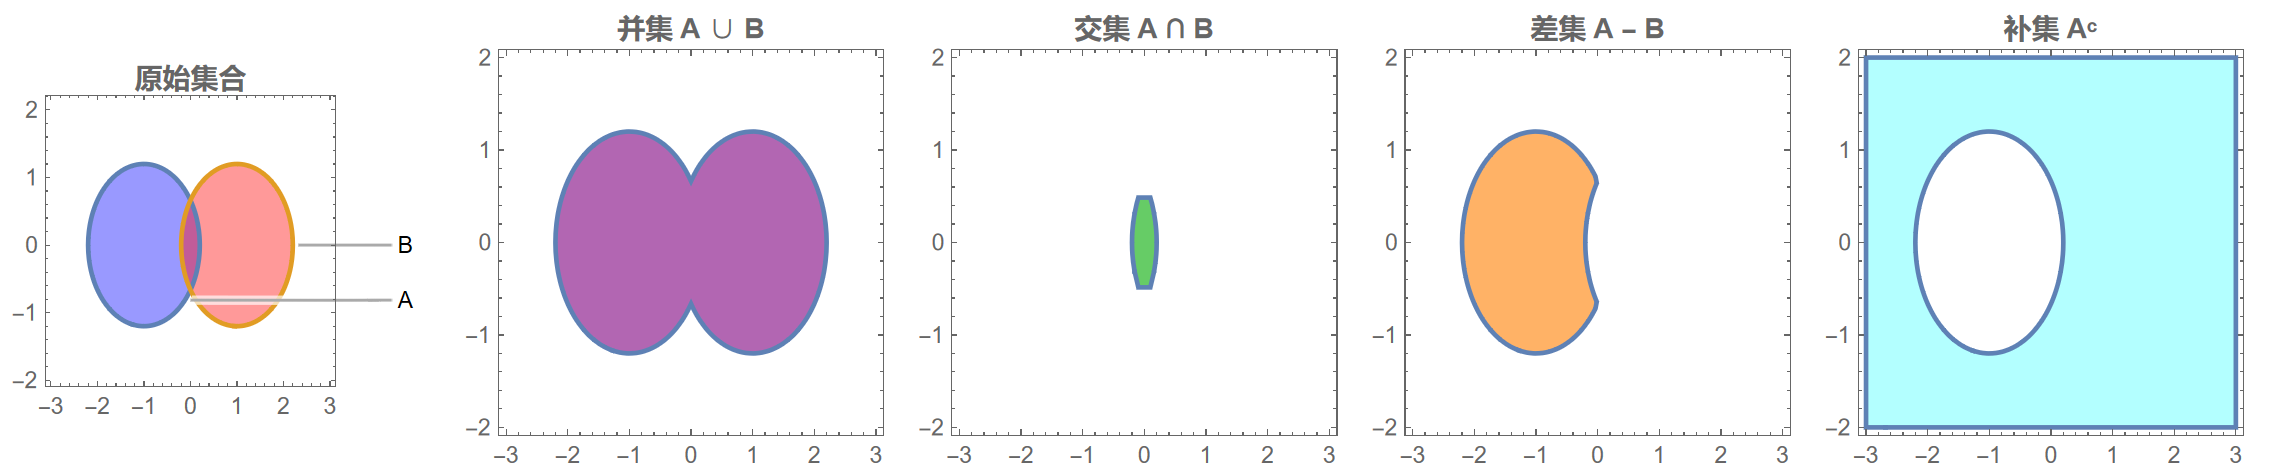
\includegraphics[width=\linewidth]{figure/C1/96aac8f9ecba0c3ccf651dd1b1ab3b43}
	\label{fig:96aac8f9ecba0c3ccf651dd1b1ab3b43}
\end{center}

\begin{proof}
	1，2是显然的，下证3\\
	先证 $A \cap(B \cup D)=(A \cap B) \cup(A \cap D)$
	\\（i）$A \cap(B \cup D) \subset(A \cap B) \cup(A \cap D)$\\
	设 $x \in A \cap(B \cup D) \Rightarrow x \in A$ 并且 $x \in B$ 或 $x \in D \Rightarrow x \in A \cap B$ 或者 $x \in A \cap D \Rightarrow x \in(A \cap B) \cup(A \cap D) \rightarrow A \cap(B \cup D) \subset(A \cap B) \cup(A \cap D)$ \\（ii）$A \cap(B \cup D) \supset( A \cap B) \cup(A \cap D)$\\
	$x \in(A \cap B) \cup(A \cap D) \Rightarrow x \in A$ 且 $x \in B$ 或 $x \in A$ 且 $x \in D \Rightarrow x$ 必 $\in A, x \in B$ 或 $x \in D \Rightarrow x \in A \cap(B \cup D) \rightarrow A \cap(B \cup D) \supset(A \cap B) \cup(A \cap D)$\\故 $A \cap(B \cup D)=(A \cap B) \cup(A \cap D)$
	
	再证 $A \cup(B \cap D)=(A \cup B) \cap(A \cup D)$
	
	$x \in A \cup(B \cap D) \Leftrightarrow x \in A$ 或$x \in B$ 并且 $x \in D \Leftrightarrow x \in A$ 或 $x \in B$ 且 $x \in A$ 或 $x \in D$
	$\Leftrightarrow x \in A \cup B$ 且 $x \in A \cup D \Leftrightarrow x \in(A \cup B) \cap(A \cup D)$
	
	
\end{proof}
\begin{proposition}
	De Morgan 公式
	$$
	(A \cup B)^C=A^C \cap B^C \quad(A \cap B)^C=A^C \cup B^C
	$$
	\label{demordan}
\end{proposition}

\begin{proof}
	先证 $(A \cup B)^C=A^C \cap B^C$
	
	$x \in(A \cup B)^c \Leftrightarrow x \notin A \cup B \Leftrightarrow x \notin A$ 且 $x \notin B \Leftrightarrow x \in A^C$ 且 $x \in B^C \Leftrightarrow x \in A^C \cap B^C$
	
	
	故 $(A \cup B)^c=A^C \cap B^C$
	
	
	
	再证明 $(A \cap B)^C=A^C\cup B^C$
	
	$ x \in(A \cap B)^C \Leftrightarrow x \notin A \cap B \Leftrightarrow x \notin A\text{或}x \notin B \Leftrightarrow x \in A^C\cup B^C$
	
	故 $(A \cap B)^C=A^C \cup B^C$
\end{proof}
\begin{corollary}
	设$\{S_{\alpha}\}$是$M$中的一组集，$\mathcal{A}$是一个指标集，那么
	\[ (\bigcap_{\alpha\in\mathcal{A}}S_{\alpha})^{C}=\bigcup_{\alpha\in\mathcal{A}}S_{\alpha}^{C}\qquad(\bigcup_{\alpha\in\mathcal{A}}S_{\alpha})^{C}=\bigcap_{\alpha\in\mathcal{A}}S_{\alpha}^{C} \]
\end{corollary}
\begin{proposition}
	\begin{enumerate}
		\item $A\setminus\varnothing=A$,$A\setminus  A=\varnothing$
		
		\item$U$是全集，$A\setminus  U=\varnothing$,$U\setminus  A=A^C$
		\item$A\setminus  B=A \cap B^c$
		\item$
		A\setminus  (B \cap C)=(A\setminus  B) \cup(A\setminus  C)
		$
		一般的，有$$X\setminus  \bigcap U_{\alpha}=\bigcup(X\setminus  U_{\alpha})$$
		
		\item$A\setminus  (B \cup C)=(A\setminus  B) \cap(A\setminus  C)$
		一般的，$$X\setminus  \bigcup U_{\alpha}=\bigcap(X\setminus  U_{\alpha})$$
		
		
		\item$A\setminus  B=\varnothing$ 当且仅当 $A \subset B$
		\item 如果 $A \subseteq B$ ，那么对于任意集合 C，有 $A\setminus  C \subseteq B\setminus  C$
		
		如果 $A \subseteq B$ ，那么 $C\setminus  B \subseteq C\setminus  A$
		
	\end{enumerate}
\end{proposition}
\begin{proof}
	\begin{enumerate}
		\item （a）$A\setminus\varnothing=A$
		
		任取 $x$ ， $x \in(A\setminus\varnothing) \Longleftrightarrow(x \in A) \textbf{且}(x \notin \varnothing) \Longleftrightarrow x \in A$ .因为 $x \notin \varnothing$ 恒真.
		所以 $A\setminus \varnothing=A$ .
		
		（b）$A\setminus A=\varnothing$
		
		任取 $x$,
		$
		x \in(A\setminus A) \Longleftrightarrow(x \in A) \textbf{且}(x \notin A) 
		$
		
		
		但 $x \in A$ 与 $x \notin A$ 不可能同时成立，故 $A\setminus A$ 不含任何元素，即 $A\setminus A=\varnothing$ 
		
		\item（a）$A\setminus U=\varnothing$
		
		任取 $x$ ，$x \in(A\setminus U) \Longleftrightarrow(x \in A) \textbf{且}(x \notin U) $
		
		因为 $U$ 是全集，所以 $x \notin U$ 恒假.
		故 $A\setminus U$ 不含任何元素，即 $A\setminus U=\varnothing$ 
		
		（b）$U\setminus A=A^c$
		
		任取 $x$，$x \in(U\setminus A) \Longleftrightarrow(x \in U) \textbf{且}(x \notin A) \Longleftrightarrow \text { True } \textbf{且}(x \notin A) \Longleftrightarrow x \notin A \Longleftrightarrow x \in A^C$
		\item
		
		任取 $x$ ，
		
		$
		x \in(A\setminus B) \Longleftrightarrow(x \in A) \textbf{且}(x \notin B) \Longleftrightarrow(x \in A) \textbf{且}\left(x \in B^C\right) \Longleftrightarrow x \in\left(A \cap B^C\right)
		$
		
		
		所以 $A\setminus B=A \cap B^C$ .
		\item 由3和\ref{demordan}易得
		
		\item 由3和\ref{demordan}易得
		\item
		 $\Rightarrow$ :假设 $A\setminus B=\varnothing$ .要证 $A \subset B$ .
		任取 $x \in A$ .若 $x \notin B$ ，则 $x \in A\setminus B$ ，与 $A\setminus B=\varnothing$ 矛盾.故 $x \in B$ .
		所以 $A \subset B$ .
		
		$\Leftarrow$ :假设 $A \subset B$ .要证 $A\setminus B=\varnothing$ .
		任取 $x \in A\setminus B$ ，则 $x \in A$ 且 $x \notin B$ .但 $A \subset B$ 意味着 $x \in A \Rightarrow x \in B$ ，矛盾.故不存在这样的 $x$ ，即 $A\setminus B=\varnothing$ .
		
		所以 $A\setminus B=\varnothing \Longleftrightarrow A \subset B$ .
		
		\item
		
		（a）如果 $A \subset B$ ，那么对于任意集合 $C$ ，有 $A\setminus C \subset B\setminus C$
		假设 $A \subset B$ .
		任取 $x \in A\setminus C$ ，则 $x \in A$ 且 $x \notin C$ .
		由 $x \in A$ 和 $A \subset B$ 得 $x \in B$ .
		
		所以 $x \in B$ 且 $x \notin C$ ，即 $x \in B\setminus C$ .
		故 $A\setminus C \subset B\setminus C$ .
		
		（b）如果 $A \subset B$ ，那么 $C\setminus B \subset C\setminus A$
		假设 $A \subset B$ .
		任取 $x \in C\setminus B$ ，则 $x \in C$ 且 $x \notin B$ .
		由 $A \subset B$ 和 $x \notin B$ 可得 $x \notin A$（因为若 $x \in A$ 则 $x \in B$ ，矛盾）.
		
		所以 $x \in C$ 且 $x \notin A$ ，即 $x \in C\setminus A$ .
		故 $C\setminus B \subset C\setminus A$ .
	\end{enumerate}
\end{proof}
我们有一下记号
	\[ S=E_1 \cup E_2 \cup \cdots E_n=\bigcup_{x=1}^n E_x\quad \bigcup_{x=1}^{+\infty} E_x\quad \bigcup_{x \in A} E_x \]
	\[T=E_1 \cap E_2 \cap \cdots \cap E_n=\bigcap_{x=1}^n E_x \quad \bigcap_{x=1}^{+\infty} E_x\quad \bigcap_{x \in A} E_x\]	
	
	
这种集合的运算性质，说明了集合构成的类加上交并补的运算可以形成一个代数结构，也就是布尔代数.
\begin{definition}
	对A，B两者的Descartes积定义为
	
	$$
	A \times B:=[(x, y): x \in A, y \in B]
	$$
	
	
	对 $A_1, \cdots, A_n$
	
	$$
	A_1 \times \cdots \times A_n:=\left[\left(x_1, \cdots, x_n\right): x_1 \in A_1, \cdots, x_n \in A_n\right]
	$$
\end{definition}
\newpage
%
% 第2节：代数结构初步
% !TEX root = ../../../main.tex
% 所属：第一部分：单变量分析学 / 第1章：实数理论——从Peano公理到实数的连续性
% 节：1.2 代数结构初步
% 正文按原文件顺序保存；由 ../chapter1.tex 调用。
\section{代数结构初步}


从自然数向有理数扩张的过程，是代数结构由低级到
高级的过程，这里对代数结构进行初步的说明.
\begin{definition}
	代数结构，是一个集合，配上一个或多个运算，并且满足一定的公理 .运算的一般形式有加法，乘法，数乘，甚至交并非的集合运算.
\end{definition}


\begin{definition}简单代数结构树状图
	
	
\end{definition} 
\begin{tikzpicture}[
	node distance=1cm and 0.8cm,  % 减小节点间距
	algNode/.style={
		draw=black,
		thick,
		rounded corners=4pt,     % 减小圆角
		minimum width=2.5cm,     % 减小宽度
		minimum height=0.8cm,    % 减小高度
		text width=2.3cm,        % 减小文本宽度
		align=center,
		font=\scriptsize         % 使用更小的字体
	},
	arrow/.style={
		-Stealth,
		thick,
		line width=0.6pt        % 减细箭头
	}
	]
	
	% 定义节点
	\node[algNode] (magma) {群胚\\集合 + 运算+封闭性};
	\node[algNode, below=of magma] (semi) {半群\\+ 结合律};
	\node[algNode, below=of semi] (monoid) {幺半群\\+ 单位元};
	\node[algNode, below left=of monoid] (group) {群\\+ 逆元};
	\node[algNode, below right=of monoid] (ring) {环\\加法阿贝尔群\\乘法半群或幺半群};
	\node[algNode, below=of group] (abelian) {阿贝尔群\\+ 交换律};
	\node[algNode, below=of ring] (commRing) {交换环\\乘法交换律};
	\node[algNode, below=of commRing] (domain) {整环\\无零因子+单位元};
	\node[algNode, below=of domain] (field) {域\\乘法逆元存在\\加法，乘法，分配公理};
	
	% 绘制箭头
	\draw[arrow] (magma) -- (semi);
	\draw[arrow] (semi) -- (monoid);
	\draw[arrow] (monoid) -- (group);
	\draw[arrow] (monoid) -- (ring);
	\draw[arrow] (group) -- (abelian);
	\draw[arrow] (ring) -- (commRing);
	\draw[arrow] (commRing) -- (domain);
	\draw[arrow] (domain) -- (field);
	
\end{tikzpicture}
\newpage

%
% 第3节：Peano公理与$\N$自然数集的构建
% !TEX root = ../../../main.tex
% 所属：第一部分：单变量分析学 / 第1章：实数理论——从Peano公理到实数的连续性
% 节：1.3 Peano公理与$\N$自然数集的构建
% 正文按原文件顺序保存；由 ../chapter1.tex 调用。
\section{Peano公理与$\N$自然数集的构建}
\begin{axiom}Peano公理\label{peano}
	\begin{enumerate}
		\item 0 是自然数.
		\item 每一个自然数 $n$ 都有且仅有一个后继 $S(n)$ ，且 $S(n)$ 也是自然数.
		
		\item 0不是任何自然数的后继.
		\item 不同的自然数有不同的后继.
		\item P(n)是一个关于自然数的命题.若 $P(0)$ 成立，对任意自然数 $k$ ，如果 $P(k)$ 能推出 $P(S(k))$ 成立，那么 $P(n)$ 对所有自然数成立.
		
		
	\end{enumerate}
	
\end{axiom}

现在 $0$ 是那个起始的数，$S(0)$ 称为 $1, S(S(0))$ 称为 2 … 以此类推得 $0,1,2,3,4$ ．．把这些不断后继得到的东西构成一个无限的集合.这个集合就是自然数集$\N$.

这样，我们就把自然数这个直观的概念建立在了不依赖直观的公理上.
\begin{definition}设$a,b\in \N$，定义$\N$上的二元运算
	\begin{itemize}
		\item 加法 
		\begin{enumerate}
			\item $ a+0=a$ 任何数加 0 等于它本身.
			\item $a+S(b)=S(a+b) $一个数加另一个数的后继，等于这两个数和的后继.
		\end{enumerate}
		\item 乘法
		\begin{enumerate}
			\item $a \cdot 0=0$
			\item$ a \cdot S(b)=a \cdot b+a$
		\end{enumerate} 
	\end{itemize}
	
	
	
\end{definition}

在这种加法和乘法的定义下，自然数集对加法能构成交换幺半群，对乘法同样.

现在，我们进述冯诺依曼对Peano公理的集合论叙述.
\begin{axiom}Peano公理的集合论叙述\label{peano2}
	\begin{enumerate}
		\item $0:=\varnothing$
		\item$S(n):=n \cup\left\{n\right\}$\\
		这样 $0:=\varnothing, 1:=S(0)=\varnothing \cup\left\{\varnothing\right\}=\left\{\varnothing\right\}=\left\{0\right\}$,
		$2:=S(1)=\left\{\varnothing\right\} \cup\{\left\{\varnothing\right\}\}=\left\{\varnothing,\left\{\varnothing\right\}\right\}=\left\{0,1\right\}\ldots$
		\item 无穷公理： $\exists$ 集合 $I$ 使得 $\varnothing\in I\text{且}x\in I\rightarrow S(x)\in I$.就称$I$为归纳集.
	\end{enumerate}
	取 $\N:=\bigcap\left\{I:I\text{是一个归纳集}\right\}$，也就是说$\N$是最小的归纳集.
\end{axiom}



说明取交的原因，集 $I=\left\{0,1,2,3,4\ldots\text{苹果},\text{苹果}^+,\text{苹果}^{++}\ldots\right\}$, 定义 0 ，苹果为起始，$S$（苹果）$=\text{苹果}^+$  ，$I$亦是归纳集，这个$I$是丑陋不堪的，不纯的，故取所有$I$的交，只留下最小的那个. \[\left\{0,1,2,3\ldots\right\}\]
现在，我们用\ref{peano2}反验\ref{peano}
\begin{proposition}
		由\ref{peano2}可以推出\ref{peano}.
\end{proposition}

\begin{proof}
	\begin{enumerate}
		\item $0=\varnothing \in$ 每一个归纳集，故 $0=\varnothing \in \bigcap I$ 成立.
		\item  $n \in \N$ 则n属于每一个归纳集，那么每一个$I$包含 $S(n)$ .
		故 $S(n) \in \N \quad$ 成立.
		\item $S(n)=n \cup\left\{n\right\}$ 包含元素 $n$ ，而 $0=\varnothing$ 不含任何元素,
		$S(n)$ 不可能是空集 ,成立.
		\item 对 $m, n \in \mathbb{N}$ ，假设 $S(m)=S(n) \Rightarrow m \cup\left\{m\right\}=n \cup\left\{n\right\}$,
		若 $m \in n$，则由 $\mathbb{N}$ 中元素的传递性（每个自然数等于其所有元素之并的子集）有 $m \subseteq n$；
		若 $m = n$，则显然 $m \subseteq n$. 无论何种情形 $m \subseteq n$.
		对称地 $n \subseteq m$，故 $m=n$ 成立.
		\item 考虑集合 $A=\left\{n \in \mathbb{N}: P(n)\text{为真}\right\}$ \\
		$P(0)$ 真，故 $0 \in A \quad$ ,若 $P(k)$ 真则 $P(S(k))$ 真，故 $k \in A \rightarrow S(k) \in A$故 $A$ 是一个归纳集 $\Rightarrow \mathbb{N} \subset A$ 又 $A \subset \N \Rightarrow A=\mathbb{N} \Rightarrow$ 对所有 $n \in \mathbb{N}$ 成立
	\end{enumerate}
\end{proof}
现在，任何关于数的理论都建立在了集合论的基础上.而我们的集合论是公理化的，严谨的，我们的数学大厦就有了坚实的地基.

%
% 第4节：等价关系，商集与$\Z$整数的构建
% !TEX root = ../../../main.tex
% 所属：第一部分：单变量分析学 / 第1章：实数理论——从Peano公理到实数的连续性
% 节：1.4 等价关系，商集与$\Z$整数的构建
% 正文按原文件顺序保存；由 ../chapter1.tex 调用。
\section{等价关系，商集与$\Z$整数的构建}
\begin{definition}
	定义一个关系是等价关系$\sim$若它满足如下条件
	\begin{enumerate}
		\item 自反性：$A \sim A$
		\item 对称性：若 $A \sim B$ 则 $B \sim A$
		\item 传递性：若 $A \sim B$ 且 $B \sim C$ 则 $A \sim C$
	\end{enumerate}
	
	
\end{definition}
\begin{definition}
	在一个集合$X$上定义一个等价关系$\sim$.
	对某一元素 $a, \left[a\right]$ 定义成所有与 $a$ 等价的元素构成的集合，也就是说
	
	$$
	[a]=\left\{x \in X: x \sim a\right\}
	$$
	
	$\left[a\right]$被称作 $a$ 的等价类.
\end{definition}

\begin{lemma}
	等价类 $[a], a \in X$ ，$[a]$ 有以下三条性质.
	\begin{enumerate}
		\item $a \in[a]$
		\item $b \in[a]$ 则 $[a]=[b]$
		\item 任意两个等价类 $[a],[b]$ 要么 $[a]=[b]$ 要么 $[a]\cap[b]=\varnothing$
	\end{enumerate}
\end{lemma}
\begin{proof}
	\begin{enumerate}
		\item $a \sim a$
		\item 任取 $x\in[a]$，即 $x\sim a$. 由 $b\in[a]$ 知 $b\sim a$，由对称性 $a\sim b$，传递性得 $x\sim b$，故 $x\in[b]$，即 $[a]\subseteq[b]$. 同理 $[b]\subseteq[a]$，故 $[a]=[b]$
		\item 若 $[a] \cap[b] \neq \varnothing$ ,设 $x \in[a] \cap[b]$ 则 $a\sim x,b\sim x,a\sim b$, 
		$[a]=[b]$
	\end{enumerate}
\end{proof}
\begin{definition}
	＂$\sim$＂是 $X$ 上的一个等价关系.由＂$\sim$＂确定的等价类构成的集合，称为 $X$ 关于 $\sim$ 的商集，记为 $X / \sim$
	
	$$
	X / \sim=\{[a]: a \in X\}
	$$
\end{definition}
现在，利用商集的概念，我们可以从自然数上构造整数.
\begin{construction}整数的构造
	$$
	\text { 令 } S=\{(a,b): a,b \in \mathbb{N}\}
	$$
	
	（虽然我们尚未定义＂减法＂，为了方便理解 $(a, b)\Leftrightarrow a-b$）\\
	在 $S$ 上定义$\sim$
	\[(a, b) \sim(c, d) \quad\text{iff}\quad a+d=b+c\]	
	
	$$
	[a+d=b+c \Leftrightarrow a-b=c-d]
	$$
	这样
	
	$$
	\Z:=S/\sim
	$$
	每个等价类 $[a, b]$ 是一个整数.
\end{construction}   



\begin{proof}
	现验证$\sim$是等价关系.
	\begin{enumerate}
		\item  自反性 $a+b=b+a \quad(a, b) \sim(a, b)$
		\item 对称性 $(a, b) \sim(c, d) \Leftrightarrow a+d=b+c \Leftrightarrow c+b=d+a \Leftrightarrow (c, d) \sim(a, b)$
		\item 
		传递性 $(a, b) \sim(c, d), ( c, d) \sim(e, f) \Leftrightarrow$
		$$
		a+d=b+c, c+f=d+e \Leftrightarrow a+f=b+e \Leftrightarrow(a, b) \sim(e, f)
		$$
	\end{enumerate}
\end{proof}

现对 $\Z$ 上的运算进行定义.\\
\begin{definition}
	加法 $[(a, b)]+[(c, d)]:=[(a+c, b+d)]$\\
	加法逆元 $-[(a, b)]:=[(b, a)]$\\
	减法 $[(a, b)]-[(c, d)]:=[(a+d, b+c)]$\\
	乘法 $[(a, b)] \cdot[(c, d)]:=[(a c+b d, a d+b c)]$\\
	通常情况下 $[(n, 0)]$ 记作 $n \quad \Rightarrow \mathbb{N} \subset \mathbb{Z}$\\
	$[(0, n)]$ 记作 $-n$\\
	$[(a,b)]$记作$a-b$\\
\end{definition}

这样，我们就严格的构造出了整数集，并且定义了其上的运算.\\
$(\Z,+)$ 是阿贝尔群，
$(\mathbb{Z}, +, \cdot)$ 是交换环\\
\begin{example}
	-2 对应 $[(3,5)],[(1,3)]$ 等,
	-4 对应 $[(1,5)],[(6,10)]$ 等
\end{example}


%
% 第5节：$\Q$有理数的构建
% !TEX root = ../../../main.tex
% 所属：第一部分：单变量分析学 / 第1章：实数理论——从Peano公理到实数的连续性
% 节：1.5 $\Q$有理数的构建
% 正文按原文件顺序保存；由 ../chapter1.tex 调用。
\section{$\Q$有理数的构建}
\begin{construction}有理数的构建
	$$
	S=\left\{(a, b): a, b \in \mathbb{Z}\text{且}b\ne0\right\}
	$$
	
	
	在 $S$ 上定义 $\sim$ 关系
	\[(a, b) \sim(c, d) \text { iff } a d=b c\]
	\[\Q:=S/\sim\]
	
\end{construction}



现验证 $\sim$ 是等价关系
\begin{proof}
	\begin{enumerate}
		\item 自反性 $(a, b) \sim(a, b) \Leftrightarrow a b=b a$
		\item   对称性 $(a, b) \sim ( c, d) \Leftrightarrow a d=b c \Leftrightarrow c b=d a$
		\[\text{故}(c, d) \sim(a, b)\]
		
		\item  传递性 $(a, b) \sim(c, d)$ 且 $(c, d) \sim(e, f)$
		
		$$
		\begin{aligned}
			& \Leftrightarrow a d=b c \text { 且 } c f=d e \\
			& \Leftrightarrow a f=b e \Leftrightarrow(a, b) \sim(e, f)
		\end{aligned}
		$$
		
	\end{enumerate}
\end{proof}
每个等价类$[(a, b)]$ 是一个有理 数.

\begin{definition}$\Q$上的运算\\
	加法 $[(a, b)]+[(c, d)]:=[( a d+b c, b d)]$\\
	加法逆元 $-[(a, b)]:=[(-a, b)]$ 或$[(a,-b)]$\\
	乘法 $[(a, b)] \cdot[c, d]:=[(a c, b d)]$\\
	乘法逆元 $[(a, b)]^{-1}=[(b, a)]$,其中$a,b\ne0$
\end{definition}

在$\Q$上$[(a, b)]$ 记作 $\dfrac{a}{b} \quad$


显然 $[(n, 1)]=n \in \mathbb{Z} \Rightarrow \mathbb{Z} \subset\Q$

$\Q$是一个数域

\begin{example}
	$$\dfrac{1}{2}=[(2,4)]=[(3,6)]=\cdots$$
	$$\dfrac{3}{5}=[(6,10)]=[(3,5)]=\cdots$$
\end{example}

%
% 第6节：数域
% !TEX root = ../../../main.tex
% 所属：第一部分：单变量分析学 / 第1章：实数理论——从Peano公理到实数的连续性
% 节：1.6 数域
% 正文按原文件顺序保存；由 ../chapter1.tex 调用。
\section{数域}
我们在这里，对域的概念加以重申.
\begin{definition}\label{1.6.1}
	一个三元组$(\F,+,\cdot)$若满足以下 11 条公理，则被称为\textbf{域}:
	\begin{enumerate}
		\item $\forall a, b \in \mathbb{F} \quad a+b \in \mathbb{F}$
		\item $\forall a, b \in \mathbb{F} \quad a+b=b+a$
		\item $\forall a, b, c \in \mathbb{F} \quad(a+b)+c=a+(b+c)$
		\item $\exists 0 \in \mathbb{F}$ 使得$a+0=a$
		\item $\exists-a \in \mathbb{F}$ 使得$-a+a=0$
		\item $\forall a, b \in \mathbb{F} \quad a b \in \mathbb{F}$
		\item $\forall a, b \in \mathbb{F} \quad a b=b a$
		\item $\forall a, b, c \in \mathbb{F} \quad(a b) c=a(b c)$
		\item $\exists 1 \in \mathbb{F}$使得 $a \cdot 1=a$
		\item $\forall a \in \F, a \neq 0 \Rightarrow \exists a^{-1} \in \F$ 使得 $a \cdot a^{-1}=1$
		\item $\forall a, b, c \in \mathbb{F} \quad(a+b) c=a \cdot c+b \cdot c$
	\end{enumerate}
	$1\sim5$称为加法公理记为$(A1)\sim(A5)$,$6\sim10$称为乘法公理记为$(M1)\sim(M5)$，11称为分配公理，记为(D)
\end{definition}
事实上，对四则运算封闭，有交换律，结合律，分配律就为域.
\begin{proposition}\label{1.6.2}
	$(A1)\sim(A5)$中有以下命题成立
	\begin{enumerate}
		\item $x+y=x+z \Rightarrow y=z$
		\item $x+y=x \Rightarrow y=0$
		\item$x+y=0 \Rightarrow y=-x$
		
		\item $-(-x)=x$
	\end{enumerate}
\end{proposition}
\begin{proof}
	$$
	\begin{aligned}
		y & =0+y=(-x+x)+y=-x+(x+y) \\
		& =-x+(x+z)=(-x+x)+z=0+z=z .
	\end{aligned}
	$$
	
	
	得证．
	
	在1中取 $z=0$ 就是2，在1中取 $z=-x$ 就是3，
	因 $-x+x=0$ ，3（用 $-x$ 代替 $x, x$ 代替 $y$ ）就能产生出4.
\end{proof}
\begin{proposition}
	$(M1)\sim(M5)$中有以下命题成立
	\begin{enumerate}
		\item $x \neq 0$ 且 $x y=x z \Rightarrow y=z$
		\item$x \neq 0$ 且 $x y=x \Rightarrow y=1$
		\item$x \neq 0$ 且 $x y=1 \Rightarrow y=\dfrac{1}{x}$
		\item $x \neq 0 \Rightarrow\left(x^{-1}\right)^{-1}=x$
	\end{enumerate}
	
\end{proposition}
\begin{proof}
	类似\ref{1.6.2}，省略
\end{proof}
\begin{proposition}\label{1.6.4}
	$\forall x, y, z \in \mathbb{F}$ ，以下命题成立
	\begin{enumerate}
		\item  $0 x=0$
		\item $x \neq 0$ 且 $y \neq 0$ 那么 $x y \neq 0$
		\item $(-x) y=-(x y)=x(-y)$
		\item $(-x)(-y)=x y$
	\end{enumerate} 
\end{proposition}
\begin{proof}
	$0 x+0 x=(0+0) x=0 x$ ．因此,有 $0 x=0$ ，而1成立
	
	
	设 $x \neq 0, y \neq 0$ 而 $x y=0$ ．于是由（a）能推出
	
	$$
	1=\left(\dfrac{1}{y}\right)\left(\dfrac{1}{x}\right) x y=\left(\dfrac{1}{y}\right)\left(\dfrac{1}{x}\right) 0=0
	$$
	
	
	矛盾．于是2成立．
	
	
	3中前一等式，可由
	
	$$
	(-x) y+x y=(-x+x) y=0 y=0
	$$
	
	
	得来；3的后半可用同样方法证明．
	
	最后，由3得
	
	$$
	(-x)(-y)=-[x(-y)]=-[-(x y)]=x y 
	$$
\end{proof}




%
% 第7节：序公理，有理数的阿基米德性和稠密性，上下确界
% !TEX root = ../../../main.tex
% 所属：第一部分：单变量分析学 / 第1章：实数理论——从Peano公理到实数的连续性
% 节：1.7 序公理，有理数的阿基米德性和稠密性，上下确界
% 正文按原文件顺序保存；由 ../chapter1.tex 调用。
\section{序公理，有理数的阿基米德性和稠密性，上下确界}
\begin{axiom}
	在集$S$上定义一种关系，名为序,记作$<$有如下性质
	
	（i）若 $x, y \in S$ ，那么在
	
	$$
	x<y \quad x=y \quad y<x
	$$
	
	
	三者中必备其一
	
	
	（ii）$x, y, z \in S \quad x<y$ 且 $y<z \Rightarrow x<z$
	
	有时用 $x>y$ 代替 $y<x$
	
	\label{1.7.1}
\end{axiom}
\begin{definition}$\N$,$\Z$,$\Q$上序的定义
	\begin{enumerate}
		\item$\N$定义序：对 $n \in \mathbb{N}$ ，规定 $S(n)>n$ 如此就定义了 $\mathbb{N}$ 上的序关系
		
		$0$ 不是任何自然数的后继，故 $0=\min\N$ 
		\item $\Z$定义序：$\Z:=\left\{[(a,b)]:a,b\in\N\right\}$
		
		若 $[(a, b)]>[(c, d)]$ 则 $a+d>b+c$
		\item 	$\Q$定义序:$\left\{[(a,b)]:a,b\in\Z\text{且}b\ne0\right\}\quad(a, b):=\dfrac{a}{b}$
		
		若 $[(a, b)]>[(c, d)]$ 则 $a d > b c$
	\end{enumerate}
	
	显然地，我们定义的序关系满足\ref{1.7.1}中的（i），（ii）
	
\end{definition}
\begin{definition}
	具有序关系 $<$ 的一个集合 $A$ 称为良序的，如果 $A$ 的任意非空子集有一个最小元.
\end{definition}
\begin{theorem}良序定理
	
	若 $A$ 是一个集合，则存在 $A$ 上的一个序关系，使 $A$ 成为一个良序集.
\end{theorem}

这个定理是1904年由 Zermelo 证明的，曾震动了数学界，并对其证明的正确性展开大量辩论.对于任意不可数集，没有一个将其良序化的构造性程序就引起了许多怀疑.在进一步分析这个证明时，我们发现只有一处可能有点问题，就是在构造的过程中包含着无穷多次选择，也就是说其做法包含了选择公理.

一些数学家曾经拒绝把选择公理作为一个结果，多少年来每涉及一个新定理就要提出这个问题：它的证明是否涉及选择公理？因为一个定理的证明中如果使用了选择公理，便会被认为基础不稳固.一般说来，时下的数学家大都已经不再有这样的烦恼了.他们把选择公理作为集合论中的一个合适的假定，良序定理也就随之得以被承认.

选择公理蕴涵良序定理的证明过于冗长（虽然不是特别困难），而且主要是逻辑学家的兴趣所在，我们略去其证明.我们承认良序定理，读者也可以将其视作另外的一个公理！

\begin{axiom}选择公理
	
	给定由两两无交的非空集合构成的一个族 $\mathcal{A}$ ，存在一个集合 $C$ ，使得 $C$ 与 $\mathcal{A}$ 的每一个元素恰好有一个公共元，即对于每一个 $A \in \mathcal{A}$ ，集合 $C \cap A$ 包含着唯一的一个元素．
\end{axiom}
\begin{definition}
	高斯取整$\left[a\right]$，是不大于 $a $的，最小的那个整数.
	
\end{definition}
\begin{proposition}
	$\Q$上的阿基米德性
	
	$x, y \in \mathbb{Q}$ 且 $x>0 \quad$ 那么 存在 $n \in \mathbb{Z}_{+} \quad$ 使
	\[	n x>y\]\label{1.7.7}
\end{proposition}

\begin{proof}
	取 $n=\left[|\dfrac{y}{x}|\right]+1$,得证.    	
	
\end{proof}
\begin{definition}\label{有序域}
	有序域是一个域 $\F$ ，又是合于下列两条件的有序集
	
	（i）当 $x, y, z \in F$ 且 $y<z$ 时，$x+y<x+z$ ；
	
	（ii）如果 $x, y \in F, x>0$ 且 $y>0$ ，那么 $x y>0$ ．
	
	如果 $x>0$ ，就说 $x$ 是正的；如果 $x<0$ ，就说 $x$ 是负的．
	
	例如，$\Q$ 是有序域．
	
\end{definition}

一个满足\ref{1.7.1}和\ref{1.7.7}的域称为 Archimedean有序域.



\begin{proposition}
	在每个有序域中，下面几条叙述都正确：
	
	（a）如果 $x>0$ ，那么 $-x<0$ ；反过来也对.
	
	（b）如果 $x>0$ 而 $y<z$ ，那么 $x y<x z$ .
	
	（c）如果 $x<0$ 而 $y<z$ ，那么 $x y>x z$ .
	
	（d）如果 $x \neq 0$ ，那么 $x^2>0$ ．特别有 $1>0$ ．
	
	（e）如果 $0<x<y$ ，那么 $0<1 / y<1 / x$ ．
\end{proposition}
\begin{proof}
	(a)如果 $x>0$ ，那么 $0=-x+x>-x+0=-x$ ，因此，$-x<0$ ．如果 $x<0$ ，那么 $0=-x+x<-x+0$ ；因此 $-x>0$ ．这就证明了（a）．
	
	（b）因为 $z>y$ ，就有 $z-y>y-y=0$ ，因此，$x(z-y)>0$ ，所以
	
	$$
	x z=x(z-y)+x y>0+x y=x y .
	$$
	
	（c）由（a）、（b）及命题\ref{1.6.4}的4
	
	$$
	-[x(z-y)]=(-x)(z-y)>0
	$$
	
	
	因此 $x(z-y)<0$ ，而得 $x z<x y$ ．
	
	（d）如果 $x>0$ ，由\ref{有序域}的第（ii）部分就得出 $x^2>0$ .
	
	如果 $x<0$ ，那么 $-x>0$ ，因此 $(-x)^2>0$ ．但是根据命题 $1.6.4(\mathrm{~d}), x^2=(-x)^2$ 
	
	因为 $1= 1^2, 1>0$ 
	
	（e）如果 $y>0$ ，而 $v \leqslant 0$ ，那么 $y v \leqslant 0$ ．但 $y \cdot(1 / y)=1>0$ ．因此 $1 / y>0$ ．类似地可得 $1 / x>0$ ．如果把不等式 $x<y$ 两端乘以正量 $(1 / x)(1 / y)$ ，就得到 $1 / y<1 / x$ 
\end{proof}




\begin{theorem}有理数的稠密性
	
	$\forall a>b \in \mathbb{Q}, \exists p \in \mathbb{Q}$ s．t．$a>p>b$ 成立
	
\end{theorem}
\begin{proof}
	取 $p=\dfrac{a+b}{2}$ 由$\Q$对加法封闭 $p \in \mathbb{Q}$,$a>p>b$成立. 
\end{proof}
\begin{definition}
	对一个已经定义了序关系集合 $S$
	
	若 $\exists \xi \in S$ s．t．$\forall x \in S$ 有 $x \leqslant \xi$ 称 $\xi$ 是 $S$ 的最大数，$\xi=\max S$
	
	若 $\exists \eta \in S$ s．t．$\forall x \in S$ 有 $\eta \leqslant x$ 称 $\eta$ 是 $S$ 的最小数 $\eta=\min S$
\end{definition}
\begin{definition}
	对一个有序集 $S$
	
	若对某 $\alpha$ ，使 $\forall x \in S$ 都有 $\alpha \geqslant x$ 则称 $\alpha$ 是 $S$ 的上界
	
	若对某 $\beta$ ，使 $\forall x \in S$ 都有 $\beta \leqslant x$ 则称 $\beta$ 是 $S$ 的下界
	
\end{definition}
\begin{definition}对一个有序集 $S$
	
	设 $\alpha$ 是 $S$ 的上界，若 $\alpha$ 满足下面的条件，则称 $\alpha$ 为 $S$ 的 上确界 记为 $\alpha=\sup S$ ：
	
	$$
	\forall \varepsilon>0 \quad \exists x \in S \text { s.t. } x>\alpha-\varepsilon
	$$
	
	
	换言之，$\sup S$是 $S$ 的最小上界
	
	$\beta$ 是$S$ 的下界，若 $\beta$ 满足下面的条件，则称 $\beta$ 为 $S$ 的下确界 记为 $\beta=\inf S$ ：
	
	$$
	\forall \varepsilon>0\quad \exists x \in S \text { s.t. } x<\beta+\varepsilon
	$$
	
	
	换言之$\inf S$是 $S$ 的最大下界
\end{definition}
\textbf{注意：}
	最大值与上确界不相同，最大值必在集合内，上确界则不一定.

\begin{definition}
	有序集 $S$ ，如果具有性质：
	
	若 $E \subset S, E$ 不空，且 $E$ 上有界时， $\sup E$ 便在 $S$ 里．就说 $S$ 有最小上界性.
	
	类似的，我们定义出最大下界性.
\end{definition}
\begin{proposition}
	设 $S$ 是具有最小上界性的有序集，$B \subset S, B$ 不空且 $B$ 下有界．令 $L$ 是 $B$ 的所有下界的集．那么
	
	$$
	\alpha=\sup L
	$$
	
	
	在 $S$ 存在，并且 $\alpha=\inf B$ ．
	特别地说就是 $\inf B$ 在 $S$ 存在
\end{proposition}

也就是说，具有最小上界性的集合一定具有最大下界性.
\begin{proof}
	因 $B$ 下有界，$L$ 不空．$L$ 刚好由这样一些 $y \in S$ 组成，它们对于每个 $x \in B$ ，满足不等式 $y \leqslant x$ ．可见每个 $x \in B$ 是 $L$ 的上界．于是 $L$ 上有界，因而我们对 $S$ 的假定意味着 $S$ 里有 $L$ 的上确界；把它叫做 $\alpha$ ．
	
	如果 $\gamma<\alpha$ ，那么 $\gamma$ 不是 $L$ 的上界，因此 $\gamma \notin B$ ．由此对于每个 $x \in B, \alpha \leqslant x$ .所以 $\alpha \in L$ .
	
	如果 $\alpha<\beta$ ，由于 $\alpha$ 是 $L$ 的上界，必然 $\beta \notin L$ ．
	我们已证明了：$\alpha \in L$ ．而当 $\beta>\alpha$ 时，就有 $\beta \notin L$ ．换句话说，$\alpha$ 是 $B$ 的下界，但若 $\beta>a, \beta$ 就不是 $B$ 的下界．这就是说 $\alpha=\inf B$ ．
\end{proof}
\begin{definition}
	确界原理是指在$S$中的一个子集，若他有上界，则必有上确界.这与$S$的最小上界性等价.
\end{definition}

\begin{definition}
	设 $A$ 和 $B$ 是分别有序关系 $<_A$ 和 $<_B$$\footnote{表示在A，B上定义的序关系}$ 的两个集合．$A \times B$ 上的全序关系定义为：当 $a_1<_A a_2$ 或者当 $a_1=a_2$ 并且 $b_1<_B b_2$ 时，
	
	$$
	a_1 \times b_1<a_2 \times b_2 .
	$$
	
	
	它称为 $A \times B$ 上的字典序关系．
\end{definition}
%
% 第8节：Dedekind分割，$\R$实数域的构造
% !TEX root = ../../../main.tex
% 所属：第一部分：单变量分析学 / 第1章：实数理论——从Peano公理到实数的连续性
% 节：1.8 Dedekind分割，$\R$实数域的构造
% 正文按原文件顺序保存；由 ../chapter1.tex 调用。
\section{Dedekind分割，$\R$实数域的构造}
\begin{definition}\label{defofded}
	在 $\Q$ 上取两个集合 $A$,$B$ 使得$\Q=A \cup B$且$\forall a \in A, b \in B$ ，$a<b$ .称由 $A, B$ 集合构成的双元组 $A \mid B$ 为 $\Q$ 的一个 Dedekind分割（或简称分割），A称为分割的下组，B称为分割的上组.
	
\end{definition}
从逻辑上讲，双元组$A|B$有 4 种情况

（a）$A$有最大数，$B$无最小数.

（b）$A$无最大数，$B$ 有最小数.

（c）$A$无最大数，$B$ 无最小数.

（d）$A$有最大数，$B$ 有最小数.

我们将证明(d)是不可能的.
\begin{proof}
	假设$\max A=a, \min B=b \in \mathbb{Q}$ ，由 $\mathbb{Q}$ 的稠密性
	
	$\exists p \in \mathbb{Q}$ 使 $a<p<b \Rightarrow p \notin A$ 且 $p \notin B$ 与 $\Q=A \cup B$ 矛盾
	
	故$(d)$不成立
	
	
\end{proof}
我们对 $(a)$,  $(b)$,$(c)$ 进行举例

\begin{example}
	（a）取 $A=\left\{x:x\leqslant a\right\}\quad B=\mathbb{Q} \backslash A=\{x \mid x>a\} \quad x \in \mathbb{Q}$
	
	用区间表示法 $A=(-\infty, a] \quad B=(a,+\infty)$
	
	$\max A=a$ 
	
	$ \quad \forall x \in A \quad x \leqslant a$ 显然的 $\quad\max A=a$
	
	$\min B  $不存在 
	
	若 $\min B=b$ 取 $\dfrac{b-a}{2} \quad b-\dfrac{b-a}{2}=\dfrac{a+b}{2}>a$
	
	可以保证 $b-\dfrac{b-a}{2}<b \quad b-\dfrac{b-a}{2} \in B$ 矛盾，故 $B$ 无最小数
	
	（b）与 （a）同理
	
	$(c)$取 $A=\left\{x :x^2<2, x \in \mathbb{Q}\right\} \quad B=\mathbb{Q} \backslash A$
	
	先证 $\forall x \in \mathbb{Q}\quad x^2 \neq 2$
	
	证明 ：
	
	$x=\dfrac{m}{n}\quad m,n$ 是既约的.若 $\left(\dfrac{m}{n}\right)^2=2 \quad m^2=2 n^2 \quad m$ 是偶的 $m=2 k \quad 2 k^2=n^2\quad n$ 亦是偶的,矛盾.
	
	$\max A \text{ 不存在}$ 
	若 $\max A$ 存在 $\max A=x \quad \exists n \in \mathbb{Z}_{+}$使 $\left(x+\dfrac{1}{n}\right)^2<2$
	
	$x^2+2 x \dfrac{1}{n}+\dfrac{1}{n^2}<2$ 取 $n>\dfrac{2x+1}{2-x^2}$ 这样 $x+\dfrac{1}{n} \in A$ 使 $x+\dfrac{1}{n}>\max A$矛盾 $ \quad \min B$ 同理
\end{example}
$\Q$上是有空隙的，这就是$\R$的构造动机.
\begin{definition}
	对 \ref{defofded}中的（a）我们说分割 $A | B$ 定义了 $\max A \in \mathbb{Q}$
	
	对 $(b)$，我们说分割 $A | B$ 定义了有理数 $\min B\in \Q$ .
	
	对（c）．$A|B$在$\Q$上无定义，我们就说 $A| B$ 定义了一个无理数.
	
	$\mathbb{R}$ 定义为所有有理数与无理数的集合.
	
\end{definition}

我们对$\R$进行考量， $\mathbb{R}$ 是否可以写成 $\Q$上 所有满足 \ref{defofded}的所有分割构成的集合.显然不能，考虑 $A \mid B$ 与 $A^{\prime} \mid B^{\prime}$ 分别满足 $(a), (b)$ 且 $A$ 的最大数与 $B$ 的最小数相等，$A \mid B$ , $A^{\prime} \mid B^{\prime}$定义了同一个有理数却是不同的分割，故我们对 \ref{defofded} 的定义做出补充.
\textbf{注：}
	在以下的叙述中，$\alpha,\beta,\gamma\in\R$,$p,q,r,s,t\in\Q$,$A,B,C\text{表示集合}$


\begin{definition}\label{1.8.5}
	分划，定义为具有以下性质的集合$\alpha\in\Q$
	
	$(I)$ $\alpha$ 不空，$\alpha \neq Q$ .
	
	$(II)$如果 $p \in \alpha, q \in Q$ 且 $q<p$ ，那么 $q \in \alpha$ .
	
	$(III)$如果 $p \in \alpha$ ，那么必有某个 $r \in \alpha$ 使得 $p<r$ .
\end{definition}
注意，（III）是说 $\alpha$ 没有最大化；（II）暗含着两件可以直接运用的事实：

如果 $p \in \alpha$ 而 $q \notin \alpha$ ，那么 $p<q$ .

如果 $r \notin \alpha$ 而 $r<s$ ，那么 $s \notin \alpha$ ．
\begin{construction}
	我们称$\Q$上所有分划$\alpha$构成的集合为$\R$.
\end{construction}


现在$\R$上定义序关系.
\begin{definition}
	规定用＂$\alpha<\beta$＂表示：$\alpha$ 是 $\beta$ 的真子集．
	
	我们来验证这符合定义 \ref{1.7.1} 的要求.
	
	如果 $\alpha<\beta$ 且 $\beta<\gamma$ ，那么显然 $\alpha<\gamma$ ．（真子集的真子集还是真子集）．对于任何一对 $\alpha, \beta$ ，显然三种关系
	
	$$
	\alpha<\beta, \quad \alpha=\beta, \quad \beta<\alpha
	$$
	
	
	之中最多有一种成立．为了证明至少有一种成立，假定前两种不成立．于是 $\alpha$ 不是 $\beta$ 的子集．由此存在一个 $p \in \alpha$ ，但 $p \notin \beta$ .如果 $q \in \beta$ ，那么（因为 $p \notin \beta$ ）$q<p$ ，因而由（II）$q \in \alpha$ ．如此就有 $\beta \subset \alpha$ ．因为 $\beta \neq \alpha$ ，所以可以断定 $\beta<\alpha$ ．
	
	于是，现在 $\R$ 是有序集了．
\end{definition}

\begin{theorem}
	有序集 $\R$ 有最小上界性．
\end{theorem}
\begin{proof}
	令 $A$ 是 $\R$ 的不空子集，且假定 $\beta \in \R$ 是 $A$ 的上界．规定 $\gamma$ 为所有 $\alpha \in A$的并．换言之，$p \in \gamma$ 当且仅当对某个 $\alpha \in A$ 有 $p \in \alpha$ ．今证 $\gamma \in \R$ ，且 $\gamma=\sup A$ ．
	
	因 $A$ 不空，存在 $\alpha_0 \in A$ ．这个 $\alpha_0$ 不空．因为 $\alpha_0 \subset \gamma, \gamma$ 也就不空．此外，$\gamma \subset \beta$ （因为每当 $\alpha \in A$ ，必然 $\alpha \subset \beta$ ）所以 $\gamma \neq \Q$ .于是 $\gamma$ 满足性质（I）．为了证明（II）和 （III），取 $p \in \gamma$ .于是有某个 $\alpha_1 \in A$ 使 $p \in \alpha_1$ .如果 $q<p$ ，那么 $q \in \alpha_1$ ，由此 $q \in \gamma$ ；这就证明了（II）．如果选得 $r \in \alpha_1$ 并且 $r>p$ ，就知道 $r \in \gamma$（因为 $\alpha_1 \subset \gamma$ ），所以 $\gamma$满足（III）.
	
	于是 $\gamma \in \R$ ．
	显然只要 $\alpha \in A$ ，必然 $\alpha \leqslant \gamma$ ．
	假定 $\delta<\gamma$ ，便有 $s \in \gamma$ 而 $s \notin \delta$ ．既然 $s \in \gamma$ ，便有某个 $\alpha \in A$ 使得 $s \in \alpha$ ．因此 $\delta<\alpha$ ，而且 $\delta$ 不是 $A$ 的上界.
	
	这就得到了所期望的结果：$\gamma=\sup A$ ．
	
	
\end{proof}
这样，$\R$满足确界原理.

接下来定义$\R$上的运算.
\begin{definition}
	如果 $ \alpha \in \R \text { 且 } \beta \in \R $ ，规定  $\alpha+\beta $ 为由所有和$ r+s$  组成的集，这里 $r \in \alpha$ , $s \in \beta$ .
	
	规定 $0^*$ 为所有负有理数组成的集．显然 $0^*$ 是一个分划．我们用 $0^*$ 当作 $0$ ，而来证明加法公理在 $\R$ 中成立.
	
\end{definition}
\begin{proof}
	
	
	$(A1)$需要证明 $\alpha+\beta$ 是分划，显然 $\alpha+\beta$ 是 $\Q$ 的不空子集．取 $r^{\prime} \notin \alpha, s^{\prime} \notin \beta$ ，那么对所有 $r \in \alpha, s \in \beta$ 来说，$r^{\prime}+s^{\prime}>r+s$ .所以 $r^{\prime}+s^{\prime} \notin \alpha+\beta$ .因此 $\alpha+\beta$ 具备性质（I）．
	
	取 $p \in \alpha+\beta$ ，则 $p=r+s$ ，这里 $r \in \alpha, s \in \beta$ ．如果 $q<p$ ，那么 $q-s<r$ ，所以 $q-s \in \alpha$ ，而 $q=(q-s)+s \in \alpha+\beta$ ，所以（II）成立．选 $t \in \alpha$ 使 $t>r$ ．于是 $p<t+s$并且 $t+s \in \alpha+\beta$ ．所以（III）成立．
	
	
	$(A2)$ $\alpha+\beta$ 是所有 $r+s$ 的集，其中 $r \in \alpha, s \in \beta$ ．据同一定义，$\beta+\alpha$ 是所有 $s+r$的集．因 $r+s=s+r$ 对所有 $r \in \Q$ 及 $s \in \Q$ 成立，所以 $\alpha+\beta=\beta+\alpha$ ．
	
	$(A3)$和上边一样，由 $\Q$ 内的结合律可以推得本条．
	
	$(A4)$如果 $r \in \alpha, s \in 0^*$ ，那么 $r+s<r$ ，因此 $r+s \in \alpha$ ．如此就有 $\alpha+0^* \subset \alpha$ ．
	为了得到相反的包含式，取 $p \in \alpha$ 又取 $r \in \alpha$ ，使 $r>p$ ．就有 $p-r \in 0^*$ 而 $p=r+(p-r) \in \alpha+0^*$ .所以 $\alpha \subset \alpha+0^*$ .于是断定 $\alpha+0^*=\alpha$ .
	
	$(A5)$固定了 $\alpha \in R$ ．令 $\beta$ 是具有以下性质的所有 $p$ 的集：
	存在 $r>0$ 使 $-p-r \notin \alpha$ ．
	换句话说，有比 $-p$ 小一点的有理数不在 $\alpha$ 内．
	今证 $\beta \in R$ 并且 $\alpha+\beta=0^{\circ}$ .
	如果 $s \notin \alpha$ 而 $p=-s-1$ ，那么 $-p-1 \notin \alpha$ ，由此 $p \in \beta$ .所以 $\beta$ 不空.如果 $q \in \alpha$ ，那么 $-q \notin \beta$ ．所以 $\beta \neq \Q$ ．因此 $\beta$ 满足（I）．
	
	取 $p \in \beta$ 及 $r>0$ ，使 $-p-r \notin \alpha$ ．若 $q<p$ ，则 $-q-r>-p-r$ ，从而 $-q-r \notin \alpha$ .于是 $q \in \beta$ ，而（II）成立.令 $t=p+(r / 2)$ ，就有 $t>p$ 且 $-t-(r / 2)=-p-r \notin \alpha$ .所以 $t \in \beta$ ．因此 $\beta$ 满足（III）．
	
	已经证明了 $\beta \in R$ .
	如果 $r \in \alpha$ 并且 $s \in \beta$ ，那么 $-s \notin \alpha$ ，因之 $r<-s, r+s<0$ .于是 $\alpha+\beta \subset 0^*$ .
	为了证明反向包含式，取 $v \in 0^*$ ，令 $w=-v / 2$ .于是 $w>0$ ，必有整数 $n$ 使得 $n w \in \alpha$ 但 $(n+1) w \notin \alpha$ .（注意，这由于 $\Q$ 有阿基米德性！）命 $p=-(n+2) w$ ，则由 $-p-w \notin \alpha$ 有 $p \in \beta$ ，也就有
	
	$$
	v=n w+p \in \alpha+\beta .
	$$
	
	
	于是 $0^* \subset \alpha+\beta$ ．
	我们断定了 $\alpha+\beta=0^{*}$ .
\end{proof}
\begin{definition}
	乘法比加法更麻烦一点，这因为负有理数的乘积是正有理数．因此，我们首先限于在 $\R^{+}$里来讨论，$\R^{+}$是所有 $\alpha \in\R$ 之合于 $\alpha>0^*$ 的集．
	
	如果 $\alpha \in R^{+}$且 $\beta \in R^{+}$，定义 $\alpha \beta$ 为所有 $p$ 组成的集，$p \leqslant r s$ ，而这里 $r \in \alpha$ ， $s \in \beta, r>0, s>0$ 是随意选定的.
	
	定义 $1^*$ 为所有 $q<1$ 组成的集．
	于是在定义 \ref{1.6.1}中，把 $\F$ 换成 $\R^{+}$，再把 $1^*$ 当作 $1$ 用时，公理（M）及（D）都成立.
	
	证法与上一条中详细给出的十分相似，因此从略．
	
	令 $\alpha 0^*=0^* \alpha=0^*$ 且令
	
	$$
	\alpha \beta= \begin{cases}(-\alpha)(-\beta) & \text { 如果 } \alpha<0^*, \quad \beta<0^*, \\ -[(-\alpha) \beta] & \text { 如果 } \alpha<0^*, \quad \beta>0^*, \\ -[\alpha \cdot(-\beta)] & \text { 如果 } \alpha>0^*, \quad \beta<0^* .\end{cases}
	$$
	
	
	就使乘法定义完全了.上式右端的乘积，是已定义了的.
	既然证了公理$（M）$在 $\R^{+}$中成立，再证它们在 $\R$ 中成立就十分简单了，只要重复应用恒等式 $\gamma=-(-\gamma)$.
	
	分配律
	
	$$
	\alpha(\beta+\gamma)=\alpha \beta+\alpha \gamma
	$$
	
	
	的证明要分情况．例如，设 $\alpha>0^*, \beta<0^*, \beta+\gamma>0^*$ ，那么 $\gamma=(\beta+\gamma)+(-\beta)$且（因已知分配律在 $\R^{+}$成立）
	
	$$
	\alpha \gamma=\alpha(\beta+\gamma)+\alpha \cdot(-\beta),
	$$
	
	
	但 $\alpha \cdot(-\beta)=-(\alpha \beta)$ ．于是
	
	$$
	\alpha \beta+\alpha \gamma=\alpha(\beta+\gamma)
	$$
	
	
	其他情形用类似的方法处理．
\end{definition}

如果 $\alpha, \beta, \gamma \in \R$ ，并且 $\beta<\gamma$ ，那么 $\alpha+\beta<\alpha+\gamma$ .

实际上，从 $\R$ 中$+$的定义显然有 $\alpha+\beta \subset \alpha+\gamma$ ；倘若 $\alpha+\beta=\alpha+\gamma$ ，消去律便暗含有 $\beta=\gamma$ ．

又随之有，$\alpha>0^*$ 当且仅当 $-\alpha<0^*$ ．

如此，$\R$是一个具有最小上界性的有序域.
\begin{proposition}
	（a）如果 $x \in \R, y \in \R$ 且 $x>0$ ，那么，必定存在正整数 $n$ ，使得
	
	$$
	n x>y .
	$$
	
	注意，这里的$n$有无穷多个.
	
	（b）如果 $x \in \R, y \in \R$ 且 $x<y$ ，那么一定存在 $p \in \Q$ 合于
	
	$$
	x<p<y .
	$$
	
	也一定存在无穷多的$t\in \R\backslash\Q$合于
	$$x<t<y$$
	
\end{proposition}

\begin{proof}
	（a）设 $\alpha=\left(A_\alpha, \mathbb{Q} \backslash A_\alpha\right)$ 是正分割，即 $\alpha>0^*$ .
	
	由序的定义， $0^* \subset \alpha$ ，所以存在某个有理数 $p \in \alpha$ 且 $p>0$
	
	取这个正有理数 $p \in \alpha, p>0$ .
	
	由有理数的阿基米德性（在 $\mathbb{Q}$ 中成立！），对任意有理数 $M$ ，$\forall x\in\beta,M>x$,存在正整数 $m$ 使得 $m p>M$ .
	
	现在给定任意实数 $\beta$ .
	$\beta$ 是一个分割，即 $\beta \subset \mathbb{Q}$ .
	取任意有理数 $M \in \mathbb{Q} \backslash \beta$
	
	存在正整数 $n$ 使得 $n p>M$ .
	
	对于 $\alpha>0^*, ~ n^* \alpha$ 定义为分割
	
	$\{r \in \mathbb{Q}:r<n a, a \in \alpha\}$ 
	
	$np\in n^*a,\textbf{且}np\in \Q$
	
	若 $q \in \beta$ ，则 $q<M<n p$ ，所以 $q \in n^* \alpha$ ，因此 $\beta \subset n^* \alpha$ .
	
	并且 $n p \in n^* \alpha$ 但 $n p \notin \beta$（因为 $n p>M$ 且 $M \notin \beta$ 推得所有大于等于 $M$ 的不在 $\beta$ 中）.
	
	所以 $\beta \subset n^* \alpha$ 且 $\beta \neq n^* \alpha$ ，即 $n^* \alpha>\beta$ .
	
	取$\cdots>n_2>n_1>n$,就有无穷多正整数$n$满足.
	
	（b）由 $x<y$ ，得 $y-x>0$ ；于是（a）提供正整数 $n$ 使得
	
	$$
	n(y-x)>1
	$$
	
	
	再应用 $(\mathrm{a})$ ，可以得到正整数 $m_1$ 及 $m_2$ ，合于 $m_1>n x . m_2>-n x$ ．于是
	
	$$
	-m_2<n x<m_1 \text {. }
	$$
	
	
	因此有正整数 $m\left(-m_2 \leqslant m \leqslant m_1\right)$ 使得
	
	$$
	m-1 \leqslant n x<m
	$$
	
	
	将这些不等式联系起来就得到
	
	$$
	n x<m \leqslant 1+n x<n y .
	$$
	
	
	因为 $n>0$ ，从而
	
	$$
	x<\dfrac{m}{n}<y .
	$$
	
	
	这就证明了（b），而 $p=m / n$ ，再在$(a,p),(p,b)$
	上找有理数不断重复，就可以找出无穷多的有理数.
	
	在 $(a, b)$ 中有 $p_1 \in \mathbb{Q} \quad a<p_1<b$
	
	$$
	b-p_1>0 \quad \exists t \in \mathbb{N}^{+} \text {s.t. } \dfrac{1}{t}<b-P_1
	$$
	
	$\sqrt{2}$ 是无理数存在 $\sqrt{2} / 2<1 \Rightarrow b-p_1>\dfrac{1}{t}>\dfrac{1}{t} \cdot \dfrac{\sqrt{2}}{2}$
	
	$$
	\Rightarrow b>p_1+\dfrac{\sqrt{2}}{2 t}>p_1>a
	$$
	
	
	由有理数构成域的性质，$p_1+\dfrac{\sqrt{2}}{2 t}$ 不是有理数，不断重复这一过程， 在 $(a, b)$ 内可取出无穷多无理数.
\end{proof}

这样我们仅仅使用了有理数上的阿基米德性，和$\sqrt{2}$的存在，就说明了$\R$上的阿基米德性和有理数与无理数在$\R$上的稠密性，这是不依赖于确界原理等实数基本定理的，仅凭戴德金分割的 定义与有理数的性质就可以构造出来.
\begin{theorem}
	Dedekind基本定理
	
	
	$\bar{A}|\bar{B}$ 为 $\mathbb{R}$ 上符合\ref{1.8.5} 的分割，在 $\mathbb{R} $ 上，只有一种可能：
	
	$\bar{A}$ 无最大值，$\bar{B}$有最小值
	
\end{theorem}
\begin{proof}
	令 $A=\bar{A} \cap Q, B=\bar{B} \cap \mathbb{Q}$
	
	$$
	\begin{aligned}
		& A \cap B=(\bar{A} \cap \mathbb{Q}) \cap(\bar{B} \cap \mathbb{Q})=\varnothing\\
		& A \cup \bar{B}=(\bar{A} \cap \mathbb{Q}) \cup(\bar{B} \cap \mathbb{Q})=\mathbb{Q}
	\end{aligned}
	$$
	
	$A \subset \bar{A}, B \subset \bar{B} ,\quad \forall a \in A \subset \bar{A}, b \in B \subset \bar{B} \quad b>a$
	
	现证$A$中无最大数：
	
	假设 $m \in A \cap \mathbb{Q}$ 是 $A \cap \mathbb{Q}$ 的最大数.
	那么 $m \in A$ ，且 $A$ 没有最大数，所以存在 $t \in A$ 使得 $t>m$ .
	由于有理数在实数中稠密，存在有理数 $q$ 满足 $m<q<t$ .
	因此 $q \in A \cap \mathbb{Q}$ .
	
	但 $q>m$ ，这与 $m$ 是 $A \cap \mathbb{Q}$ 的最大数矛盾.
	
	故 $A|B$ 是 $\Q$ 的一个分割
	
	对$A|B$有两种情况
	\begin{enumerate}
		\item $A$ 无最大数，$B$有最小数.
		\item $A$无最大数，$B$无最小数
		
	\end{enumerate}
	
	
	
	
	
	对1断言$\bar{A}$无最大数，$\bar{B}$有最小数$b_0$.
	
	如若不然，假设$\bar{B}$无最小数
	
	$\quad \exists b \in \bar{B}$ 且 $b<b_0$ .
	
	因为$ b_0 \in  B \subset \bar{B}$,故$ \exists r \in \mathbb{Q}$ s．t．$b<r<b_0$
	
	因为$b \in \bar{B}$,所以 $b \notin \bar{A}$且$r \in \bar{B} \Rightarrow r \notin A \Rightarrow r \in B \quad$ 矛盾
	
	再假设 $\bar{A}$ 有最大数，设 a 为 $\bar{A}$ 的最大数 .
	
	$a \in \bar{A} \Rightarrow a \notin \bar{B} ,\quad b_0$ 为 $\bar{B}$ 的最小数 $b_0>a$.
	
	$\exists r \in \mathbb{Q}, a < r<b_0$ .因 $r<b_0 \quad r \notin \bar{B}, r \in \bar{A}$ 矛盾
	
	对（2）．$A|B$定义了一个无理数 $c \in \mathbb{R}=\bar{A} \cup \bar{B}$
	
	
	
	有一种情况
	
	$c \in \bar{B} \Rightarrow$ $\bar{A}$无最大，$\bar{B}$有最小 $c$.
	
	若 $\bar{B}$ 无最小数，$\exists b \in \bar{B}$ s．t．$b <c\Rightarrow \exists r \in \mathbb{Q}$ ，s．t．$b<r<c \quad r \in \bar{B}$
	
	且 $r \in \mathbb{Q} \Rightarrow r \in B$ 与 $B$ 中元素小于 $c$ 矛盾
	
	若$\bar{A}$ 有取大数记为 $a^{\prime},  a^{\prime} \in \bar{A} $ 
	
	$\exists r \in \mathbb{Q}$ 使得$a^{\prime}<r<c \quad r \notin \bar{A} \textbf{也} r \notin 6\bar{B} 
	$矛盾.
	
	
\end{proof}
这样，我们就完成了 Dedekind基本定理的证明.

可以看到的是，在Dedekind基本定理的证明中，我们使用了实数的稠密性，这由确界定理推出，也就说明确界原理是能够推出Dedekind基本定理的，在第二章中，我们将看到，这两条定理是实数基本定理的其中之二，现在我们可以试着证明由戴德金基本定理能够推出确界原理.
\begin{proof}
	设 $S$ 为有上界集合．若 $\exists \eta \in S, \exists \eta$ 为 $S$ 的上界，那么容易知道，$\eta=\sup S$ ．
	
	否则，记 $S$ 的上界集为 $B$ ，令 $A=\R \backslash B$ ．显然 $S \subseteq A$ ，且容易知道，$A| B$ 构成 $\R$ 的一个分划．由 Dedekind 准则和所定义的分化可知，$B$ 必有最小元 $c$ ．若 $\exists \varepsilon_0>0$ ，使得 $\forall x \in S$ 都有 $x \leqslant c-\varepsilon_0$ ，则 $c-\varepsilon_0 \in B$ ．因为 $c$ 是 $B$ 的最小元，所以 $c-\varepsilon_0 \geqslant c$ 矛盾．故 $\forall \varepsilon>0$ ， $\exists x \in S$ ，使得 $x>c-\varepsilon_0$ ，即 $c$ 为 $S$ 的上确界．
\end{proof}
\begin{proposition}
	\label{1.8.13}
	对于每个实数 $x>0$ 及每个整数 $n>0$ ，有一个且仅有一个实数 $y>0$ ，使得 $y^n=x$ .
\end{proposition}


此数 $y$ 记作 $\sqrt[n]{x}$ 或 $x^{\dfrac{1}{n}}$ .
\begin{proof}
	这样的 $y$ 最多有一个：这是显然的，因为由 $0<y_1<y_2$ 就有 $y_1^n<y_2^n$ ．
	
	设由满足 $t^n<x$ 的所有正实数 $t$ 组成集 $E$ ．
	如果 $t=x /(1+x)$ ，那么 $0<t<1$ ．由此 $t^n<t<x$ ．所以 $t \in E$ 而 $E$ 不空．
	如果 $t>1+x$ ，那么 $t^n \geqslant t > x$ ，因此 $t \notin E$ ．所以 $1+x$ 是 $E$ 的上界．
	于是，$\R$的最小上界性保证
	
	$$
	y=\sup E
	$$
	
	
	存在．为了证明 $y^n=x$ ，我们证明无论是 $y^n<x$ 或是 $y^n>x$ 都会导致矛盾．
	
	恒等式 $b^n-a^n=(b-a)\left(b^{n-1}+b^{n-2} a+\cdots+a^{n-1}\right)$ 当 $0<a<b$ 时，能产生不等式
	
	$$
	b^n-a^n<(b-a) n b^{n-1}
	$$
	
	
	假如 $y^n<x$ ，选一个 $h$ ，要它满足 $0<h<1$ 和
	
	$$
	h<\dfrac{x-y^n}{n(y+1)^{n-1}}
	$$
	
	
	置 $a=y, b=y+h$ ，就得
	
	$$
	(y+h)^n-y^n<h n(y+h)^{n-1}<h n(y+1)^{n-1}<x-y^n
	$$
	
	
	于是 $(y+h)^n<x$ 而 $y+h \in E$ ．因 $y+h>y$ ，这与 $y$ 是 $E$ 的上界这事实矛盾．
	假如 $y^n>x$ ，置
	
	$$
	k=\dfrac{y^n-x}{n y^{n-1}}
	$$
	
	
	于是 $0<k<y$ ．如果 $t \geqslant y-k$ ，便可以推知
	
	$$
	y^n-t^n \leqslant y^n-(y-k)^n<k n y^{n-1}=y^n-x
	$$
	
	
	所以 $t^n>x$ ．于是 $t \notin E$ ．因之 $y-k$ 是 $E$ 的上界．
	但 $y-k<y$ ，这与 $y$ 是 $E$ 的最小上界的事实矛盾．
	由此 $y^n=x$ .证明完毕.
	
\end{proof}
\begin{corollary}
	如果 $a, b$ 是正实数，而 $n$ 是正整数，那么
	
	$$
	(a b)^{\dfrac{1}{n}}=a^{\dfrac{1}{n}} b^{\dfrac{1}{n}}
	$$
	
	
	
\end{corollary}
\begin{proof}
	命 $\alpha=a^{1 / n}, \beta=b^{1 / n}$ ．由于乘法可以交换，所以
	
	$$
	a b=\alpha^n \beta^n=(\alpha \beta)^n
	$$
	
	
	由\ref{1.8.13}所说的惟一性可以断定：$(a b)^{1 / n}=\alpha \beta=a^{1 / n} b^{1 / n}$ ．
	
	
\end{proof}
\begin{proposition}
	我们指出实数和十进小数之间的关系
	
	设 $x>0$ 是实数，令 $n_0$ 是合于 $n_0 \leqslant x$ 的最大整数.（注意，$n_0$ 的存在性，依赖于 $\R$ 的阿基米德性.）在取定 $n_0, n_1, \cdots, n_{k-1}$ 之后，令 $n_k$ 是合于
	
	$$
	n_0+\dfrac{n_1}{10}+\cdots+\dfrac{n_k}{10^k} \leqslant x .
	$$
	
	
	的最大整数．令 $E$ 是由数
	$$
	n_0+\dfrac{n_1}{10}+\cdots+\dfrac{n_k}{10^k} \quad(k=0,1,2, \cdots)
	$$
	组成的集，于是 $ x=\sup E .x $的十进小数展开式是 
	$n_0 \cdot \overline{n_1 n_2 n_3 \cdots}$
\end{proposition}
\begin{proposition}
	有理数是有限或循环小数,无理数是无限不循环小数
\end{proposition}


注：以下的证明中，使用了带余除法存在性的定理，证明移步至代数或数论的笔记中.
\begin{proof}
	$r \in \mathbb{Q}, q, p \in \mathbb{Z} $ 且 $(p, q)=1$ 现假定 $p, q$ 都大于 0 ，若小于 0 ，整体取负号就移入正号上的讨论.
	
	$$
	\exists a_0, r_0 \in \mathbb{Z}\quad0 \leqslant r_0<q \text { s.t. } p=q \cdot a_0+r_0
	$$
	
	
	小数部分由 $r_0$ 开始. $a_0$ 是 $\dfrac{p}{q}$ 的整数部分
	对 $n \geqslant 0$
	
	$$
	10 r_n=q \cdot a_{n+1}+r_{n+1} \quad 0 \leqslant r_{n+1}<9
	$$
	
	$a_{n+1}$ 是小数点后第 $n+1$ 位数字，$r_{n+1}$ 是新的余数.
	
	若某 $r_k=0$ 则 $10 r_k=0 \quad a_{k+1}=r_{k+1}=0 \rightarrow$ 小数点后终止 ，也就是有限小数
	
	若所有 $r_n \neq 0$ ，则 $r_n \in\{1,2, \cdots, q-1\}$ 只有 $q-1$ 种可能的非零余数
	
	第 $q$ 个余数 $r_q$ 之前一共 $q+1$ 个余数 $r_0, r_1, \cdots, r_q$ 由抽屉原理，
	$q+1$ 个余数中必然存在 $i<j$ s．t．$r_i=r_j$
	
	设$i$是最小的这样一个指标，
	
	$$
	\begin{gathered}
		10 r_i=q a_{i+1}+r_{i+1} \\
		10 r_j=qa_{j+1}+r_{j+1} \\
		r_i=r_j\text{故} \quad 10 r_i=10 r_j \Leftrightarrow q\left(a_{i+1}-a_{j+1}\right)=r_{j+1}-r_{i+1}
	\end{gathered}
	$$
	
	由于 $0 \leqslant r_{i+1}, r_{j+1}<q \quad$ 有 $\left|r_{j+1}-r_{i+1}\right|<q$ ，而左边是 $q$ 的倍数，只能为0.
	
	故 $a_{i+1}=a_{j+1}, r_{i+1}=r_{j+1}$，
	
	如此 $a_{i+k}=a_{j+k}, r_i+R=r_j+R$ 对所有 $k \geqslant 0$ 成立，
	
	因此从$i$开始，小数部分呈现同期 $j-i$ 的循环.
	
	反向来说明有限小数.
	
	$$
	x=a_0 .\overline{a_1 \cdot \cdots a_n}
	$$
	
	
	可以写成
	
	$$
	\dfrac{10^na_0+10^{n-1}a_1+\cdots+a_n}{10^n}
	$$
	
	无限循环小数
	
	$$
	\begin{aligned}
		& \quad y=a_{0}. a_1 \cdot a_n \dot{b}_1 \cdots \dot{b}_m \\
		& y \cdot 10^{m+n}-y 10^n=\overline{a_0 a_1 \cdots a_n b_1 \cdots b_m}-\overline{a_0 \cdots a_n} \\
		& y=\dfrac{\overline{a_0 \cdots a_n b_1 \cdots b_m}-\overline{a_0 \cdot a_n}}{10^{m+n}-10^n}
	\end{aligned}
	$$
	对无理数，因无理数与有理数构成所有实数，有限或循环小数与无限不循环小数也构成所有实数，而有理数与有限或循环小数等同，故无理数是无限不循环小数.
\end{proof}
\begin{definition}广义实数系由实数域 $\R$ 及两个符号 $+\infty$ 与 $-\infty$ 组成．我们保留 $\R$ 中原来的顺序，并对任何 $x \in \R$ 规定
	
	$$
	-\infty<x<+\infty
	$$
	
\end{definition}
显然，$+\infty$ 是广义实数系的每个子集的上界，且每个不空子集有最小上界．例如，如果 $E$ 是一个不空实数集，它在 $R$ 中不上有界，那么在广义实数系中 $\sup E=+\infty$ .

对于下界可完全一样进行讨论.

广义实数系不成域，但习惯上作如下的约定：
\begin{itemize}
	\item 如果 $x$ 是实数，那么
	
	$$
	x+\infty=+\infty, x-\infty=-\infty \quad \dfrac{x}{+\infty}=\dfrac{x}{-\infty}=0
	$$
	\item 如果 $x>0$ ，那么 $x \cdot(+\infty)=+\infty, x \cdot(-\infty)=-\infty$ 
	\item 如果 $x<0$ ，那么 $x \cdot(+\infty)=-\infty, x \cdot(-\infty)=+\infty$ .
\end{itemize}
在chapter2中，我们给出$+\infty,-\infty$的定义.
%
% 第9节：映射，有限集和可数集
% !TEX root = ../../../main.tex
% 所属：第一部分：单变量分析学 / 第1章：实数理论——从Peano公理到实数的连续性
% 节：1.9 映射，有限集和可数集
% 正文按原文件顺序保存；由 ../chapter1.tex 调用。
\section{映射，有限集和可数集}
\begin{definition}
	考虑两个集 $A$ 和 $B$ ，它们的元素可以是任何东西．
	
	假定对于 $A$的每个元素 $x$ ，按照某种方式，与集 $B$ 的一个元素联系着，这个元素记作 $f(x)$ ；那么，就说 $f$ 是从 $A$ 到 $B$ 的一个函数（或将 $A$ 映入 $B$ 内的一个映射）．集 $A$ 叫做 $f$ 的定义域（或者说 $f$ 定义在 $A$ 上），而元素 $f(x)$ 叫做 $f$ 的值．$f$ 的一切值的集叫做 $f$ 的值域．
	
	定义域$A$,值域$B$,这种关系(法则)$f$,三者的整体，我们称为一个函数.
	
\end{definition}
\begin{definition}
	设 $A$ 和 $B$ 是两个集，$f$ 是 $A$ 到 $B$ 内的一个映射．
	
	如果 $E \subset A$ ，对于一切 $x \in E$ ，元素 $f(x)$ 所成的集定义为 $f(E)$ .我们称 $f(E)$ 为 $E$ 在 $f$ 之下的象．
	
	按这个记法来说，$f(A)$ 就是 $f$ 的值域．显然 $f(A) \subset B$ ．如果 $f(A)=B$ ，就说 $f$ 将 $A$ 映满 $B$ .
	
	$E \subset B$ 时，$f^{-1}(E)$ 表示一切合于 $f(x) \in E$ 的 $x \in A$ 所成的集．称 $f^{-1}(E)$ 为 $E$ 在 $f$ 之下的逆象. $y \in E$ 时，$f^{-1}(E)$ 是 $A$ 中一切合于 $f(x)=y$ 的元素 $x$ 所成的集．
	
	如果 $f^{-1}(y)$ 对于每个 $y \in B$ 至多含有 $A$ 中的一个元素，那么就称 $f$ 是 $A$ 到 $B$内的 $1-1$（一对一的）映射．这句话也可以表述如下：如果对于 $x_1 \in A, x_2 \in A$ ，当 $x_1 \neq x_2$ 时，$f\left(x_1\right) \neq f\left(x_2\right)$ ，那么 $f$ 就是 $A$ 到 $B$ 内的一个 $1-1$ 映射．
	
	
	$\left(x_1 \neq x_2\right.$ 表示 $x_1$ 和 $x_2$ 是不同的元素；否则就记作 $x_1=x_2$ .）
\end{definition}
\begin{definition}
	若存在A到B上的$1-1$映射，A,B之间就存在一个 等价关系.
\end{definition}
\begin{definition}
	对于任意正整数 $n$ ，令 $J_n$ 表示 $1,2, \cdots, n$ 所成的集，令 $\Z_+$ 表示全体正整数所成的集．设 $A$ 是任意一个集．我们说
	\begin{enumerate}
		\item $A$ 是有限的，如果对于某个 $n, A \sim J_n$（空集也认为是有限集）
		\item $A$ 是无限的，如果 $A$ 不是有限的．
		\item $A$ 是可数的，如果 $A \sim \Z_+$
		\item $A$ 是不可数的，如果 $A$ 既不是有限的，也不是可数的．
		\item $A$ 是至多可数的，如果 $A$ 或为有限或为可数的．
	\end{enumerate}
	
\end{definition}
\begin{definition}
	定义在一切正整数的集 $\Z_+$ 上的函数叫做一个序列，如果对于 $n \in \Z_+, f(n)=x_n$ ，习惯上就把序列 $f$ 用符号 $\left\{x_n\right\}$ 来表示，或者用 $x_1, x_2, x_3, \cdots$来表示．$f$ 的值，即元素 $x_n$ ,叫做这个序列的项．设 $A$ 是一个集并且对一切 $n \in \Z_+$ ， $x_n \in A$ ，那么 $\left\{x_n\right\}$ 就叫做 $A$ 里的一个序列，或者叫做 $A$ 的元素的一个序列．
	
	
\end{definition}
注意，一个序列的项 $x_1, x_2, x_3, \cdots$ 不一定各不相同
\begin{proposition}
	可数集 $A$ 的每个无限子集也是可数集．
\end{proposition}

\begin{proof}
	设 $E \subset A$ 并且 $E$ 是无限集．把 $A$ 的元素 $x$ 排成一个不同元素的序列 $\left\{x_n\right\}$ .按以下方式作序列 $\left\{n_k\right\}$ ：
	
	令 $n_1$ 是使 $x_{n_1} \in E$ 的最小正整数．当 $n_1, \cdots, n_{k-1}(k=2,3,4, \cdots)$ 选定以后，令 $n_k$ 是大于 $n_{k-1}$ 并且使 $x_{n_k} \in E$ 的最小正整数．
	
	令 $f(k)=x_{n_k}(k=1,2,3, \cdots)$ ，我们便得到了 $E$ 和 $\Z_+$ 之间的一个 $1-1$ 对应．
\end{proof}
\begin{proposition}
		设 $\left\{E_n\right\} n=1,2,3, \cdots$ 是可数集组成的序列，令
	
	$$
	S=\bigcup_{n=1}^{\infty} E_n,
	$$
	
	
	那么 $S$ 是可数的．\label{uniofconset}
\end{proposition}

\begin{proof}
	把每个集 $ E_n$   排成一个序列 $\left\{x_{n _k}\right\}, k=1,2,3, \cdots $，而来考虑无限阵列 
	\begin{center}
		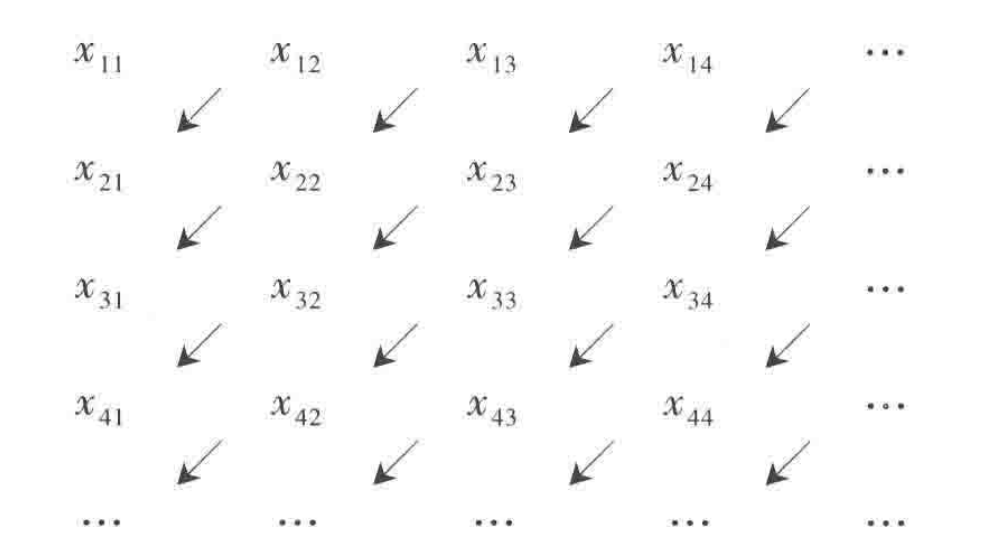
\includegraphics[width=0.7\linewidth]{figure/C1/8e9c0c930834b91d997911bb6ae34b5a}
	\end{center}
	

	把所有的元素排列成
	
	$$
	x_{11}, x_{12}, x_{21}, x_{13}, x_{22}, x_{31}, x_{14}, x_{23}, x_{32}, x_{41}, \cdots,
	$$
	这些集 $E_n$ 的任何两个如果有公共元素，那么这些公共元素将在上面的排列中不止出现一次.因此一切正整数的集里有一个子集 $T\subset\Z_+$ 使得 $S \sim T$ ，这就证明了 $S$ 是至多可数的.因为 $E_1 \subset S$ ，而 $E_1$ 是无限的，所以 $S$ 也是无限的，从而是可数的.
	
\end{proof}
\begin{corollary}\label{1.9.8}
	假定 $A$ 是至多可数的，并且对应于每个 $\alpha \in A$ 的 $B_\alpha$ 是至多可数
	的．令
	
	$$
	T=\bigcup_{\alpha \in A} B_\alpha
	$$
	
	
	那么 $T$ 是至多可数的．
\end{corollary}
$T$是\ref{uniofconset}中的$S$的一个子集.
\begin{proposition}
	\label{couofdes}
	$A_i$ 是可数集，$B_n=A_1 \times \cdots \times A_n$ 那么 $B_n$ 是可数的.
	
	换言之，可数集的有限次 Descartes 积是可数的
\end{proposition}

\begin{proof}
	$n=2$ 时 $ B_2=A_1 \times A_2=\left\{\left(x_1, x_2\right): x_1 \in A_1, x_2 \in A_2\right\}$
	
	令 $a_{i j}=\left(x_{1 i} , x_{2 j}\right)$ 由\ref{1.9.8}中的构造. $B_2$ 可数
	
	设 $B_{k-1}$ 可数
	
	$$
	B_k=A_1 \times \cdots A_{k-1} \times A_k=B_{k-1} \times A_k
	$$
	可数.
\end{proof}

\begin{remark}
	可数集的可数 次 Descartes 积不是可数的，使用下一节的定义，这个集合与 $\mathbb{R}$ 等势.
\end{remark}

下面我们考察一些集合的可数性.
\begin{proposition}
		$\Z,\Q$可数，$\R$不可数.
\end{proposition}

\begin{proof}
	对$\Z$ $f(n)=\left\{\begin{array}{cc}\dfrac{n}{2} & n \text { 是偶数 } \\ -\dfrac{n-1}{2} & n \text { 是奇数 }\end{array}\right.$
	
	对$\Q$由\ref{couofdes}可得
	
	对 $\mathbb{R}$ ,只需证 $(0,1)$ 内的所有实数不可数.
	
	如若不然，将所有 $(0,1)$ 内的实数用十进小数列出
	
	$$
	\begin{aligned}
		& r_1=0 . \overline{a_{11} a_{12} a_{13} a_{14}} \\
		& r_2=0 . \overline{a_{21} a_{22} a_{23} a_{24}} \cdots \\
		& r_3=0 . \overline{a_{31} a_{32} a_{33} a_{34}} \cdots \\
		& r_4=0 . \overline{a_{41} a_{42} a_{43} a_{44}} \cdots
	\end{aligned}
	$$
	
	
	构造 $b=0 . \overline{b_1 b_2 b_3 b_4} \cdots$ 使得 $b_1 \neq a_{11}, b_2 \neq a_{22}, b_3 \neq a_{33} \cdots$
	比如记 
	
	$\ b_n=\left[\begin{array}{ll}1 & \text { 若 }a_{n n} \neq 1 \\ 2 &\text { 若 } a_{n n}=1\end{array}\right.$
	
	$b$这个实数不在列表当中 ，矛盾，故不可数.
\end{proof}


\begin{lemma}(像-原像引理)
	设 \( f: X \to Y \) 是两个集合 \( X \) 和 \( Y \) 之间的映射，则以下命题成立：
	
	\begin{enumerate}
		\item[(0)]
		\begin{tabular}{ll}
			(a) & \( X = f^{-1}(Y) \) \\
			(b) & \( \varnothing  = f^{-1}(\varnothing ) \)
		\end{tabular}
		
		\item[(1)]
		\begin{tabular}{ll}
			(a) & 对于任意子集 \( U \subset X \)，有 \( U \subset f^{-1}(f(U)) \) \\
			(b) & 进一步，如果 \( f \) 是单射，则有 \( U = f^{-1}(f(U)) \)
		\end{tabular}
		
		\item[(2)]
		\begin{tabular}{ll}
			(a) & 对于任意子集 \( V \subset Y \)，有 \( V \supset f(f^{-1}(V)) \) \\
			(b) & 进一步，如果 \( f \) 是满射，则有 \( V = f(f^{-1}(V)) \)
		\end{tabular}
		
		\item[(3)] 对于 \( X \) 的任意一族子集 \(\{U_i\}_{i \in I}\)，有
		\[ f\left(\bigcup_{i \in I} U_i\right) = \bigcup_{i \in I} f(U_i) \]
		
		\item[(4)] 对于 \( X \) 的任意一族子集 \(\{U_i\}_{i \in I}\)，有
		\[ f\left(\bigcap_{i \in I} U_i\right) \subseteq \bigcap_{i \in I} f(U_i) \]
		
		\item[(5)]
		\begin{tabular}{ll}
			(a) & 对于任意子集 \( U \subset X \)，有 \( f(X \setminus U) \supset f(X) \setminus f(U) \) \\
			(b) & 进一步，如果 \( f^{-1}(f(U)) = U \)，则有 \( f(X \setminus U) = f(X) \setminus f(U) \)
		\end{tabular}
		
		\item[(6)] 对于 \( Y \) 的任意一族子集 \(\{V_i\}_{i \in I}\)，有
		\[ f^{-1}\left(\bigcup_{i \in I} V_i\right) = \bigcup_{i \in I} f^{-1}(V_i) \]
		
		\item[(7)] 对于 \( Y \) 的任意一族子集 \(\{V_i\}_{i \in I}\)，有
		\[ f^{-1}\left(\bigcap_{i \in I} V_i\right) = \bigcap_{i \in I} f^{-1}(V_i) \]
		
		\item[(8)] 对于任意子集 \( V \subset Y \)，有
		\[ f^{-1}(Y \setminus V) = X \setminus f^{-1}(V) \]
	\end{enumerate}
\end{lemma}

\begin{proof}
	\begin{enumerate}
		\item[(0)]
		\begin{enumerate}
			\item[(a)] 对于任意 \( x \in X \)，有 \( f(x) \in Y \)，因此 \( x \in f^{-1}(Y) \)，所以 \( X \subseteq f^{-1}(Y) \)。又因为 \( f^{-1}(Y) \subseteq X \)，所以 \( X = f^{-1}(Y) \)。
			
			\item[(b)] 因为 \( f^{-1}(\emptyset) = \{ x \in X \mid f(x) \in \emptyset \} = \emptyset \)，所以 \( \emptyset = f^{-1}(\emptyset) \)。 \end{enumerate}
		
		\item[(1)]
		\begin{enumerate}
			\item[(a)] 对于任意 \( x \in U \)，有 \( f(x) \in f(U) \)，因此 \( x \in f^{-1}(f(U)) \)，所以 \( U \subseteq f^{-1}(f(U)) \)。
			
			\item[(b)] 如果 \( f \) 是单射，且 \( x \in f^{-1}(f(U)) \)，则 \( f(x) \in f(U) \)，即存在 \( u \in U \) 使得 \( f(x) = f(u) \)。由于 \( f \) 是单射，所以 \( x = u \in U \)，因此 \( f^{-1}(f(U)) \subseteq U \)。结合 (1a) 可得 \( U = f^{-1}(f(U)) \)。 \end{enumerate}
		
		\item[(2)]
		\begin{enumerate}
			\item[(a)] 对于任意 \( y \in f(f^{-1}(V)) \)，存在 \( x \in f^{-1}(V) \) 使得 \( f(x) = y \)。根据定义，\( f(x) \in V \)，所以 \( y \in V \)，因此 \( f(f^{-1}(V)) \subseteq V \)。
			
			\item[(b)] 如果 \( f \) 是满射，对于任意 \( y \in V \)，存在 \( x \in X \) 使得 \( f(x) = y \)。因为 \( y \in V \)，所以 \( x \in f^{-1}(V) \)，因此 \( y \in f(f^{-1}(V)) \)，所以 \( V \subseteq f(f^{-1}(V)) \)。结合 (2a) 可得 \( V = f(f^{-1}(V)) \)。 \end{enumerate}
		
		\item[(3)] 对于任意 \( y \in f\left(\bigcup_{i \in I} U_i\right) \)，存在 \( x \in \bigcup_{i \in I} U_i \) 使得 \( f(x) = y \)。这意味着存在 \( i \in I \) 使得 \( x \in U_i \)，因此 \( y \in f(U_i) \)，所以 \( y \in \bigcup_{i \in I} f(U_i) \)。反之，对于任意 \( y \in \bigcup_{i \in I} f(U_i) \)，存在 \( i \in I \) 使得 \( y \in f(U_i) \)，因此存在 \( x \in U_i \) 使得 \( f(x) = y \)，所以 \( y \in f\left(\bigcup_{i \in I} U_i\right) \)。因此等式成立。
		
		\item[(4)] 对于任意 \( y \in f\left(\bigcap_{i \in I} U_i\right) \)，存在 \( x \in \bigcap_{i \in I} U_i \) 使得 \( f(x) = y \)。对于任意 \( i \in I \)，有 \( x \in U_i \)，因此 \( y \in f(U_i) \)，所以 \( y \in \bigcap_{i \in I} f(U_i) \)。
		
		\item[(5)]
		\begin{enumerate}
			\item[(a)] 对于任意 \( y \in f(X) \setminus f(U) \)，存在 \( x \in X \) 使得 \( f(x) = y \) 且 \( x \notin U \)，即 \( x \in X \setminus U \)，因此 \( y \in f(X \setminus U) \)。
			
			\item[(b)] 如果 \( f^{-1}(f(U)) = U \)，对于任意 \( y \in f(X) \setminus f(U) \)，假设 \( y \in f(U) \)，则存在 \( x \in U \) 使得 \( f(x) = y \)，这意味着 \( x \in f^{-1}(f(U)) = U \)，矛盾。因此 \( f(X \setminus U) \subseteq f(X) \setminus f(U) \)。结合 (5a) 可得 \( f(X \setminus U) = f(X) \setminus f(U) \)。 \end{enumerate}
		
		\item[(6)] 对于任意 \( x \in f^{-1}\left(\bigcup_{i \in I} V_i\right) \)，有 \( f(x) \in \bigcup_{i \in I} V_i \)，即存在 \( i \in I \) 使得 \( f(x) \in V_i \)，因此 \( x \in f^{-1}(V_i) \)，所以 \( x \in \bigcup_{i \in I} f^{-1}(V_i) \)。反之亦然，因此等式成立。
		
		\item[(7)] 对于任意 \( x \in f^{-1}\left(\bigcap_{i \in I} V_i\right) \)，对于任意 \( i \in I \)，有 \( f(x) \in V_i \)，因此 \( x \in f^{-1}(V_i) \)，所以 \( x \in \bigcap_{i \in I} f^{-1}(V_i) \)。反之亦然，因此等式成立。
		
		\item[(8)] 对于任意 \( x \in f^{-1}(Y \setminus V) \)，有 \( f(x) \in Y \setminus V \)，即 \( f(x) \notin V \)，因此 \( x \notin f^{-1}(V) \)，所以 \( x \in X \setminus f^{-1}(V) \)。反之亦然，因此等式成立。
	\end{enumerate}
\end{proof}
现在，我们用集合的方式，对映射再此定义，同时我们可以定义出二元运算的集合论形式.
\begin{definition}指派法则是两个集合的笛卡儿积 $C \times D$ 的一个子集 $r$，该子集满足这样的条件：$C$ 的每一个元素最多是 $r$ 中一个有序偶对的第一个坐标.
	
	这样，$C \times D$ 的一个子集 $r$ 如果满足
	
	$$
	\left[(c, d) \in r \text { 并且 }\left(c, d^{\prime}\right) \in r\right] \Longrightarrow\left[d=d^{\prime}\right] \text {, }
	$$
	则成为一个指派法则．我们可以将 $r$ 设想成一种指派方法，为 $C$ 的元素 $c$ 配置 $D$ 的满足 $(c, d) \in r$的元素 $d$ .
	
	对于一个指派法则 $r$ ，其定义域是由 $r$ 的元素的所有第一个坐标组成的 $C$ 的子集，其值域是由 $r$ 的元素的所有第二个坐标组成的 $D$ 的子集，即
	
	$r$ 的定义域 $=\{c $: 存在 $d \in D$ ，使得 $(c, d) \in r\}$ ，
	
	$r$ 的值域 $=\{d $ :存在 $c \in C$ ，使得 $(c, d) \in r\}$ ．
	
	函数$f$是指派法则$r$,与其定义域和值域三者组成的整体.
\end{definition}
\begin{definition}
	集合  $A $ 中的一个二元运算是将  $A \times A$ 映到  $A  $中的一个函数$  f $
\end{definition}
这样无论是整个实数的体系，还是函数的定义，或者是加减乘除的二元运算，都建立在公理化的集合论之上.
%
% 第10节：集合的势
% !TEX root = ../../../main.tex
% 所属：第一部分：单变量分析学 / 第1章：实数理论——从Peano公理到实数的连续性
% 节：1.10 集合的势
% 正文按原文件顺序保存；由 ../chapter1.tex 调用。
\section{集合的势}
\begin{definition}
	设 $A$, $B$ 是两个集合. 如果存在 $A$ 到 $B$ 的双射（即一一对应），则称 $A$ 与 $B$ \textbf{等势}，记作 $A \approx B$.
	
	集合的\textbf{势}（或基数）是集合在等势关系下的等价类，记作 $\operatorname{Card}(A)$ 或 $|A|$.
\end{definition}

容易验证 $\approx$ 是一个等价关系. 有限集的势就是其元素的个数；无限集的势则刻画了"无穷"的不同层次.

\begin{definition}
	设 $A$, $B$ 为集合. 若存在 $A$ 到 $B$ 的单射，则称 $A$ 的势\textbf{小于等于} $B$ 的势，记作 $\operatorname{Card}(A) \leqslant \operatorname{Card}(B)$.
	
	若 $\operatorname{Card}(A) \leqslant \operatorname{Card}(B)$ 且 $\operatorname{Card}(A) \neq \operatorname{Card}(B)$，则称 $A$ 的势\textbf{严格小于} $B$ 的势，记作 $\operatorname{Card}(A) < \operatorname{Card}(B)$.
\end{definition}

\begin{theorem}(Cantor--Bernstein 定理)
	若 $\operatorname{Card}(A) \leqslant \operatorname{Card}(B)$ 且 $\operatorname{Card}(B) \leqslant \operatorname{Card}(A)$，则 $\operatorname{Card}(A) = \operatorname{Card}(B)$.
\end{theorem}
这个证明我们在将来的拓扑学笔记中给出
\begin{definition}
	可数无穷集的势记作 $\aleph_0$（阿列夫零）. 即
	\[
	\aleph_0 := \operatorname{Card}(\N).
	\]
	势不超过 $\aleph_0$ 的集合称为\textbf{至多可数}的.
\end{definition}

由前几节的讨论，我们有
\[
\operatorname{Card}(\Z) = \operatorname{Card}(\Q) = \aleph_0.
\]
更一般地，可数个可数集的并仍是可数的.

\begin{definition}
	实数集 $\R$ 的势称为\textbf{连续统势}，记作 $\mathfrak{c}$（即 $2^{\aleph_0}$）.
	\[
	\mathfrak{c} := \operatorname{Card}(\R) = 2^{\aleph_0}.
	\]
\end{definition}

我们已经用对角线法证明了 $\R$ 不可数，因此 $\aleph_0 < \mathfrak{c}$.

\begin{theorem}[Cantor]
	对任意集合 $A$，有 $\operatorname{Card}(A) < \operatorname{Card}(\mathcal{P}(A))$，其中 $\mathcal{P}(A)$ 是 $A$ 的幂集. 特别地，
	\[
	\aleph_0 < 2^{\aleph_0} < 2^{2^{\aleph_0}} < \cdots,
	\]
	即存在无穷多个不同的无穷基数.
\end{theorem}

\textbf{注：}
	是否存在一个集合，其势严格介于 $\aleph_0$ 与 $\mathfrak{c}$ 之间？Cantor 猜测不存在这样的集合，即 $\mathfrak{c} = \aleph_1$（$\aleph_1$ 是大于 $\aleph_0$ 的最小基数）. 这一猜想称为\textbf{连续统假设}（Continuum Hypothesis, CH）.
	
	G\"{o}del (1940) 证明了 CH 与 ZFC 公理系统相容（不可证伪）；Cohen (1963) 证明了 CH 的否定也与 ZFC 相容（不可证明）. 因此，CH 独立于 ZFC —— 在标准的集合论公理下，它既不能被证明，也不能被否定.



	有限集的势显然小于 $\aleph_0$. 因此基数的无界递增链为
	\[
	0, 1, 2, \ldots, n, \ldots < \aleph_0 < 2^{\aleph_0} < 2^{2^{\aleph_0}} < \cdots.
	\]


%
% 第11节：复数域
% !TEX root = ../../../main.tex
% 所属：第一部分：单变量分析学 / 第1章：实数理论——从Peano公理到实数的连续性
% 节：1.11 复数域
% 正文按原文件顺序保存；由 ../chapter1.tex 调用。
\section{复数域}
\begin{definition}
	
	在 $ \mathbb{R} \times \mathbb{R}$  上定义如下等价关系 
	$$(a, b) \sim(c, d):=a=c \text { 且 } b=d$$
	$$\mathbb{C}:=\mathbb{R} \times \mathbb{R} / \sim$$
	
	
	设 $x=(a, b), y=(c, d)$ 是两个复数．我们定义：
	
	$$
	\begin{aligned}
		x+y & =(a+c, b+d) \\
		x y & =(a c-b d, a d+b c)
	\end{aligned}
	$$
	$(\C,+,\cdot)$是一个域，$(1,0)$视作$1$,$(0,0)$视作$0$
	$$\dfrac{1}{x}:=(\dfrac{a}{a^2+b^2},-\dfrac{b}{a^2+b^2})$$
	规定$(0,1)=i,(0,1)\cdot(0,1)=i^2=(-1,0)$
	
	习惯上，记$(a,b)=a+bi$
\end{definition}
\begin{definition}
	如果 $a, b$ 是实数，而 $z=a+b i$ ，就把复数 $\bar{z}=a-b i$ 叫做 $z$ 的共轭数.数 $a, b$ 分别叫做 $z$ 的实部和虚部.
	
	有时写成
	
	$$
	a=\operatorname{Re}(z), \quad b=\operatorname{Im}(z)
	$$
	
	
\end{definition}
\begin{proposition}
	\label{proofcon}
	如果 $z$ 及 $w$ 是复数，那么
	
	（a）$\overline{z+w}=\bar{z}+\bar{w}$ ，
	
	（b）$\overline{z w}=\bar{z} \cdot \bar{w}$ ，
	
	（c）$z+\bar{z}=2 \operatorname{Re}(z), \quad z- \bar{z}=2 i \operatorname{Im}(z)$ ．
	
	（d）$z \bar{z}$ 是实数且是正数（除了 $z=0$ 时）
\end{proposition}

\begin{proof}
	证（a），（b），（c）都十分明显，今证（d）．将 $z$ 写成 $z=a+b i$ ，并注意 $z \bar{z}= a^2+b^2$ .就行了.
\end{proof}
\begin{definition}
	如果 $z$ 是一复数，它的绝对值 $|z|$ 是 $z \bar{z}$ 的非负平方根；即 $|z|=(z \bar{z})^{1 / 2}$ .
	
\end{definition}

\begin{remark}
	当 $x$ 是实数时 $\bar{x}=x$ ，因此，$|x|=\sqrt{x^2}$ ．于是，如果 $x \geqslant 0,|x|=x$ ：如果 $x<0,|x|=-x$
\end{remark} 
\begin{proposition}
		设 $z$ 和 $w$ 都是复数，那么
	
	（a）$|z|>0$ 除非 $z=0,|0|=0$ ，
	
	（b）$|\bar{z}|=|z|$ ，
	
	（c）$|z w|=|z||w|$ ，
	
	（d）$|\operatorname{Re} z| \leqslant|z|$ ，
	
	（e）$|z+w| \leqslant|z|+|w|$ ．
\end{proposition}

\begin{proof}
	（a）及（b）是显然的．设 $z=a+b i, w=c+d i, a, b, c, d$ 为实数．
	
	于是
	
	$$
	\begin{aligned}
		|z w|^2 & =(a c-b d)^2+(a d+b c)^2 \\
		& =\left(a^2+b^2\right)\left(c^2+d^2\right)=|z|^2|w|^2
	\end{aligned}
	$$
	
	
	或 $|z w|^2=(|z||w|)^2$ .由定理$1.8.12$所说的惟一性，便能推得（c）.
	
	今证（d），注意 $a^2 \leqslant a^2+b^2$ ，由此，
	
	$$
	|a|=\sqrt{a^2} \leqslant \sqrt{a^2+b^2} .
	$$
	
	
	今证（e），注意 $\bar{z} w$ 是 $z \bar{w}$ 的共轭数，所以 $z \bar{w}+\bar{z} w=2 \operatorname{Re}(z \bar{w})$ .由此，
	
	$$
	\begin{aligned}
		|z+w|^2 & =(z+w)(\bar{z}+\bar{w})=\bar{z}+z \bar{w}+\bar{z} w+w \bar{w} \\
		& =|z|^2+2 \operatorname{Re}(z \bar{w})+|w|^2 \\
		& \leqslant|z|^2+2|z \bar{w}|+|w|^2 \\
		& =|z|^2+2|z||w|+|w|^2=(|z|+|w|)^2 .
	\end{aligned}
	$$
	
	
	两端开平方即得（e）.
\end{proof}
\begin{proposition}
	(Cauchy-Schawtz不等式)
	如果 $a_1, a_2, \cdots, a_n$ 及 $b_1, b_2, \cdots, b_n$ 都是复数，那么
	
	$$
	\left|\sum_{j=1}^n a_j \bar{b}_j\right|^2 \leqslant \sum_{j=1}^n\left|a_j\right|^2 \sum_{j=1}^n\left|b_j\right|^2 .
	$$
	\label{Cauchy-Schawtz不等式}
\end{proposition}

\begin{proof}
	设 $A=\Sigma\left|a_j\right|^2, B=\Sigma\left|b_j\right|^2, C=\Sigma a_j \bar{b}_j$（在本证明的所有和中，$j$ 遍历 $1, \cdots, n$ 诸值）.
	
	如果 $B=0$ ，那么 $b_1=\cdots=b_n=0$ ，而定理的结论是明显的.
	
	因此，可假定 $B>0$ ．由定理 \ref{proofcon}，有
	
	$$
	\begin{aligned}
		\sum\left|B a_j-C b_j\right|^2 & =\sum\left(B a_j-C b_j\right)\left(B \bar{a}_j-\bar{Cb_j}\right) \\
		& =B^2 \sum\left|a_j\right|^2-B \bar{C} \sum a_j \bar{b}_j-B C \sum \bar{a}_j b_j+|C|^2 \sum\left|b_j\right|^2 \\
		& =B^2 A-B|C|^2 \\
		& =B\left(A B-|C|^2\right) .
	\end{aligned}
	$$
	
	
	因第一个和中的每一项非负，而知
	
	$$
	B\left(A B-|C|^2\right) \geqslant 0 .
	$$
	
	
	由 $B>0$ 推得 $A B-|C|^2 \geqslant 0$ ．这就是要证的不等式．
\end{proof}
%
% 第12节：欧氏空间
% !TEX root = ../../../main.tex
% 所属：第一部分：单变量分析学 / 第1章：实数理论——从Peano公理到实数的连续性
% 节：1.12 欧氏空间
% 正文按原文件顺序保存；由 ../chapter1.tex 调用。
\section{欧氏空间}
\begin{definition}
	$\R^k$定义为k个$\R$的笛卡尔积.
	
	$\R^k=\left\{\boldsymbol{x}:\boldsymbol{x}=\left(x_1, x_2, \cdots, x_k\right),x_1,x_2,\cdots,x_k\in\R\right\}$
	
	称$\R^k$中的元素为向量，
	
	如果  $\boldsymbol{y}=\left(y_1, \cdots, y_k\right)$ 
	,而$\alpha\in\R$令
	
	$$
	\begin{aligned}
		\boldsymbol{x}+\boldsymbol{y} & =\left(x_1+y_1, x_2+y_2, \cdots, x_k+y_k\right), \\
		\alpha \boldsymbol{x} & =\left(\alpha x_1, \alpha x_2, \cdots, \alpha x_k\right)
	\end{aligned}
	$$
	
	
	于是 $\boldsymbol{x}+\boldsymbol{y}\in \R^k, \alpha \boldsymbol{x} \in \R^k$ .这就规定了向量的加法及向量的数乘.显然的，这两种运算满足交换律，结合律和分配律.而使 $\R^k$ 成为实数域上的向量空间. $\R^k$ 的零元是一切坐标都是 0 的点 $\mathbf{0}$ ．
\end{definition}
\begin{definition}
	$\boldsymbol{x}$ 与 $\boldsymbol{y}$ 的＂内积＂为
	
	$$
	\boldsymbol{x} \cdot \boldsymbol{y}=\sum_{i=1}^k x_i y_i
	$$
	
	
	又定义 $\boldsymbol{x}$ 的范数为
	
	$$
	|\boldsymbol{x}|=(\boldsymbol{x} \cdot \boldsymbol{x})^{1 / 2}=\left(\sum_{i=1}^k x_i^2\right)^{1 / 2} .
	$$
\end{definition}
具有上述的内积和范数的 $\R^k$ 称为 $k$ 维欧氏空间．
\begin{proposition}设 $\x, \y, \z \in \R^k, \lambda, \mu \in \R$
	\begin{enumerate}
		\item $\x\cdot\y=\y\cdot\x$
		\item $(\lambda\x+\mu\y)\cdot\z=\lambda\x\cdot\z+\mu\y\cdot\z$
		\item $(\x\cdot\y)^2\leqslant(\x\cdot\x)(\y\cdot\y)$
		
	\end{enumerate}
\end{proposition}
\begin{proof}
	1,2两条由内积的定义是显然的，3是\ref{Cauchy-Schawtz不等式}在实数下向量形式的表述，由\ref{Cauchy-Schawtz不等式}显然.
\end{proof}
\begin{proposition}设 $\x, \y, \z \in \R^k$ ，而 $\alpha$ 是实数．那么
	\begin{enumerate}
		\item$|\boldsymbol{x}| \geqslant 0$ 
		\item$|\boldsymbol{x}|=0$ 当且仅当; $\boldsymbol{x}=\mathbf{0}$ ；
		\item$|\alpha \boldsymbol{x}|=|\alpha||\boldsymbol{x}|$ ；
		\item$|\boldsymbol{x} \cdot \boldsymbol{y}| \leqslant|\boldsymbol{x}|| \boldsymbol{y} \mid$
		\item$|\boldsymbol{x}+\boldsymbol{y}| \leqslant|\boldsymbol{x}|+|\boldsymbol{y}|$
		\item$|\x-\z| \leqslant|\x-\y|+|\y-\z|$ ．
	\end{enumerate}
\end{proposition}
\begin{proof}
	1,2,3都显然成立．4是 Schwarz 不等式的直接结果,等价于1.12.3的第三条，由4
	$$
	\begin{aligned}
		|x+y|^2 & =(x+y) \cdot(x+y) \\
		& =x \cdot x+2 x \cdot y+y \cdot y \\
		& \leqslant|x|^2+2|x| y\left|+|y|^2\right. \\
		& =(|x|+|y|)^2
	\end{aligned}
	$$
	在5中用 $\x-\y$ 代 $\x$ ，用 $\y-\z$ 代 $\y$ 就得到5．
	
	
\end{proof}
%
